\documentclass[12pt,notitlepage]{report}
\usepackage{cite}					%bibliography
\usepackage{mathptmx}				%Times New Roman
\usepackage{geometry}				% Margins
 \geometry{
 a4paper,
 total={210mm,297mm},
 left=20mm,
 right=20mm,
 top=20mm,
 bottom=20mm,
 bindingoffset=0mm
 }
\usepackage[utf8]{inputenc}
\usepackage{tikz}
\usepackage{float}
\usepackage[ruled,vlined,noend]{algorithm2e}
\usepackage{caption}
\usepackage{subcaption}
\usepackage[english]{babel}
\usepackage{amssymb}
\usepackage{amsmath}
\DeclareMathOperator*{\argmin}{argmin}

\usepackage{tikz-uml}
\usepackage{graphicx}
\usepackage{fancybox}
\newcommand{\shadowpicture}[1]{%
  \shadowsize=1pt
  \fboxrule=0pt
  \fboxsep=0pt
  \color{gray}
  \shadowbox{\fboxsep=6pt\fcolorbox{white}{white}{#1}}
  \normalcolor
}

\usepackage{xcolor}
\usepackage{listings}
\lstset{language=java, frame=single,framesep=\fboxsep,framerule=\fboxrule,
rulecolor=\color{red},backgroundcolor=\color{yellow!5},basicstyle=\footnotesize\tt,tabsize=1,
numbersep=5mm, numbers=left,numberstyle=\footnotesize,keywordstyle=\color{blue}\sf,identifierstyle=\color{magenta}}

\usepackage{todonotes}

\begin{document}

%%%%%%%%%%%%%%%%%%%%%%%%%%%%%%%%%%%%%%%%%%%%%%%%%%%%%%%%%%%%%%%%%%%%%%%%
% Title


\pagestyle{empty}

\hfill{\LARGE \bf Oliver Freeman}

\vspace*{60mm}
\begin{center}
\Huge
{\bf A comparison of \\Any-Angle Pathfinding Algorithms \\for Virtual Agents} \\
\vspace*{5mm}
Computer Science: Part II \\
\vspace*{5mm}
Clare College \\
\vspace*{5mm}
\today  % today's date
\end{center}

\cleardoublepage

%%%%%%%%%%%%%%%%%%%%%%%%%%%%%%%%%%%%%%%%%%%%%%%%%%%%%%%%%%%%%%%%%%%%%%%%%%%%%%
% Proforma, table of contents and list of figures

\setcounter{page}{1}
\pagenumbering{roman}
\pagestyle{plain}

\chapter*{Proforma}

{\large
\begin{tabular}{ll}
Name:               & \bf Oliver Freeman                      \\
College:            & \bf Clare College                    \\
Project Title:      & \bf A comparison of Any-Angle Pathfinding\\ 
                    & \bf Algorithms for Virtual Agents \\
Examination:        & \bf Computer Science Tripos: Part II, May 2014        \\
Word Count:         & \bf ????\footnotemark[1]\\
Project Originator: & \bf Oliver Freeman                   \\
Supervisor:         & \bf Dr R. J. Gibbens                   \\ 
\end{tabular}
}

\footnotetext[1]{This word count was computed by {\tt detex diss.tex | wc -w}.} 


\section*{Original Aims of the Project}

\todo{Original Aims of the Project \ldots}

\section*{Work Completed}

\todo{Work completed \ldots}

\section*{Special Difficulties}

None
 
\newpage
\section*{Declaration}

I, Oliver Freeman of Clare College, being a candidate for Part II of the Computer
Science Tripos, hereby declare that this dissertation and the work described in it are my own work,
unaided except as may be specified below, and that the dissertation
does not contain material that has already been used to any substantial
extent for a comparable purpose.

\bigskip
\leftline{Signed [signature]}

\medskip
\leftline{Date [date]}

\cleardoublepage

\tableofcontents

\listoffigures

\listofalgorithms

\newpage
\section*{Acknowledgements}

\todo{Acknowledgments: including citations? \ldots}

%%%%%%%%%%%%%%%%%%%%%%%%%%%%%%%%%%%%%%%%%%%%%%%%%%%%%%%%%%%%%%%%%%%%%%%
% now for the chapters

\cleardoublepage        % just to make sure before the page numbering
                        % is changed

\setcounter{page}{1}
\pagenumbering{arabic}
\pagestyle{headings}

\chapter{Introduction}

\section{Motivation}

Finding short and realistic-looking paths through maps with arbitrarily placed obstacles is one of the central problems in artificial intelligence for games and robotics. Figure 1.1 (a) shows a grid-based map, consisting of free cells and blocked cells. Figure 1.1 (b) shows the shortest path through this map between the $start$ and the $goal$.\\

\noindent
However, pathfinding algorithms operate on graphs. A graph representation of this map is shown in figure 1.1 (c) --- each node in the graph represents a coordinate on the map, and an agent can travel directly between any two nodes connected by an edge. Figure 1.1 (d) shows the shortest path through the graph --- however, this is clearly longer than the optimum path through the map, shown in figure 1.1 (b).\\

\begin{figure}[h]
\centering
    \begin{tikzpicture}[scale=1.1,line width=0.5pt]
    
    \node (a) at (0,4) {
    \begin{tikzpicture}[scale=1.1,line width=0.5pt]
      \filldraw[color=black!60,fill=black!40] (1,1) rectangle (2,3); 
      \draw[color=black!60] (0,0) grid (3,3);
      \draw[black] (0,0) -- (3,0);
      \draw[black] (0,0) -- (0,3);
      \draw[black] (3,3) -- (3,0);
      \draw[black] (3,3) -- (0,3);
      
      \node[below] at (1.5,0) {(a)};
      \end{tikzpicture}
      };
      
     \node (b) at (6,4) {
      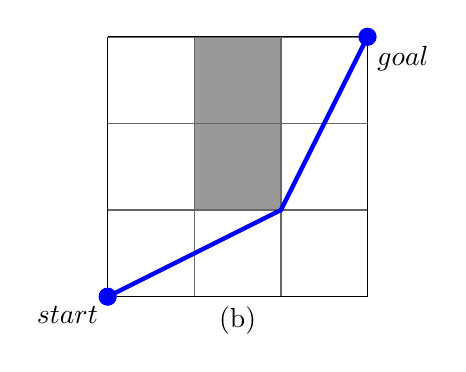
\begin{tikzpicture}[scale=1.1,line width=0.5pt]
      \filldraw[color=black!60,fill=black!40] (1,1) rectangle (2,3); 
      \draw[color=black!60] (0,0) grid (3,3);
      \draw[blue, ultra thick] (0,0) -- (2,1) -- (3,3); 
      
      \draw[black] (0,0) -- (3,0);
      \draw[black] (0,0) -- (0,3);
      \draw[black] (3,3) -- (3,0);
      \draw[black] (3,3) -- (0,3);
      
      \node[below right] at (3,3) {$goal$};
      \fill[blue] (3,3) circle (3pt);
      \node[below left] at (0,0) {$start$};
      \fill[blue] (0,0) circle (3pt);
      
      \node[below] at (1.5,0) {(b)};
      
      \end{tikzpicture}
      };
      
      \node (c) at (0,0) {
      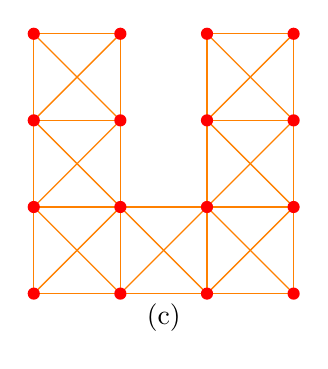
\begin{tikzpicture}[scale=1.1,line width=0.5pt]

     \draw[orange] (0,0) grid (3,3);
     
     \foreach \x in {0,1,2} {
        \foreach \y in {0,1,2} {
          \pgfmathparse{int(\x + 1)};
          \let\xa\pgfmathresult;
          \pgfmathparse{int(\y + 1)};
          \let\ya\pgfmathresult;
          \draw[orange] (\x,\y) -- (\xa,\ya);
        }
      }
  
      \foreach \x in {0,1,2} {
        \foreach \y in {1,2,3} {
          \pgfmathparse{int(\x + 1)};
          \let\xa\pgfmathresult;
          \pgfmathparse{int(\y - 1)};
          \let\ya\pgfmathresult;
          \draw[orange] (\x,\y) -- (\xa,\ya);
        }
      }
      
       \filldraw[color=orange,fill=white] (1,1) rectangle (2,3);
      \draw[white, ultra thick] (1,2) -- (2,2);
      \draw[white, ultra thick] (1,3) -- (2,3);

      \foreach \x in {0,1,2,3} {
        \foreach \y in {0,1,2,3} {
          \fill[red] (\x,\y) circle (2pt);
        }
      }
      
      \node[below] at (1.5,0) {(c)};
      \end{tikzpicture}
      };
      
      \node (d) at (6,0) {
      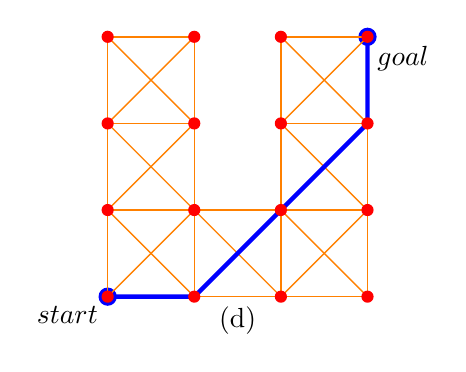
\begin{tikzpicture}[scale=1.1,line width=0.5pt]
    
      \fill[blue] (3,3) circle (3pt);
      \fill[blue] (0,0) circle (3pt);
      \draw[orange] (0,0) grid (3,3);
  
      \foreach \x in {0,1,2} {
        \foreach \y in {0,1,2} {
          \pgfmathparse{int(\x + 1)};
          \let\xa\pgfmathresult;
          \pgfmathparse{int(\y + 1)};
          \let\ya\pgfmathresult;
          \draw[orange] (\x,\y) -- (\xa,\ya);
        }
      }
  
      \foreach \x in {0,1,2} {
        \foreach \y in {1,2,3} {
          \pgfmathparse{int(\x + 1)};
          \let\xa\pgfmathresult;
          \pgfmathparse{int(\y - 1)};
          \let\ya\pgfmathresult;
          \draw[orange] (\x,\y) -- (\xa,\ya);
        }
      }

      \node[below right] at (3,3) {$goal$};
      \node[below left] at (0,0) {$start$};

      \draw[blue, ultra thick] (0,0) -- (1,0) -- (3,2) -- (3,3);
      
      \filldraw[color=orange,fill=white] (1,1) rectangle (2,3);
      \draw[white, ultra thick] (1,2) -- (2,2);
      \draw[white, ultra thick] (1,3) -- (2,3);

      \foreach \x in {0,1,2,3} {
        \foreach \y in {0,1,2,3} {
          \fill[red] (\x,\y) circle (2pt);
        }
      }
      \node[below] at (1.5,0) {(d)};
      \end{tikzpicture}
      };
      
      \node[left] at (-2,0.2) {node};
      \draw[->] (-2,0.2) -- (-1.55,0.75);
      \node[right] at (2,0.2) {edge};
      \draw[->] (2,0.2) -- (1.2,0.4);
      
      \node[left] at (-2,4.7) {free cell};
      \draw[->] (-2,4.7) -- (-1,5.3);
      \node[right] at (2,4) {blocked cell};
      \draw[->] (2,4) -- (0,4.4);
      
    \end{tikzpicture}
  \caption[Shortest paths through maps and graphs]{Shortest path through a map vs. shortest path through the graph representing the map}
 \label{fig:fart}
\end{figure}

\noindent
The structure of this graph is based on the grid structure of the map. If a different graph representation was chosen then a shorter path could have been achieved, but in general such a graph would require many more nodes and edges which would cause exponentially increasing memory requirements and search-space size. This dissertation will investigate various algorithms that aim to find a near-optimal path through a map while using space-efficient grid-based graph like that shown in figure 1.1(c).\\

\section{Related work}

{\em A*} is well known algorithm that finds optimal paths through graphs. Applying a post-processing step to smoothe paths returned by {\em A*} to make them more optimal in relation to maps is technique that has been used since the earliest video games\cite{Thorpe84}, but most of the research into more advanced any-angle pathfinding algorithms have taken place in the last half decade. \\

\noindent
Ferguson and Stentz's paper on {\em Field D*}\cite{FergusonStentz06} in 2006 was followed by a significant contribution to the field by Nash and Koenig et al., who published papers on {\em Theta*}\cite{Daniel10} and {\em Lazy Theta*}\cite{Nash10} in 2010. In 2011, Yap's paper on {\em Block A*}\cite{Yap11} introduced the concept of pre-calculating solutions to sub-maps to speed up execution.\\

\noindent
Studies such as Nash and Koneig's article in {\em Artificial Intelligence Magazine}\cite{Nash11} have been conducted that compare a selection of these any-angle pathfinding algorithms, though the only established authority that utilises empirical data on {\em Block A*} is Yap's own work\cite{Yap11}, which compares only {\em A*}, {\em Theta*} and {\em Block A*}.

\section {Project goals}

\todo{Therefore, in this project I am aiming to reconcile the gaps in the literature by...?}

\noindent
The goals of this project are to:

\begin{itemize}
\item create an algorithm simulation environment that enables intuitive and informative comparison of the performance of the most prominent any-angle path-finding algorithms;
\item use statistical analysis to present conclusions on the suitability of these algorithms to different path-finding situations.
\end {itemize}

\cleardoublepage


\chapter{Preparation} 

\section{Introduction to any-angle pathfinding}

This section formally introduces the concept of maps and describes how graphs are created from maps. It then defines the any-angle path-finding problem. A formal mathematical framework is defined throughout this section so that the any-angle pathfinding algorithms can be explained using a unifying graph-theoretic approach. Such an approach has not been attempted in any of the published papers on any-angle pathfinding algorithms.

\subsection{Map}

A map $M$ of size $N^{2}$ is a square region in two-dimensional space $[0,N]^{2} \subseteq \mathbb{R}^{2}$, where $N \in\mathbb{Z}$ and $N > 0$. A location on the map can be specified with a coordinate $(x,y) \in M$.\\

\noindent
The map is logically divided into a grid of $N^{2}$ cells of size $1 \times 1$, where cell $C_{i,j}$ includes all locations $(x,y) \in M$ where $i \leq x \leq i+1$ and $j \leq y \leq j+1$, and each cell is either `free' or `blocked'.\\

\begin{figure}
\centering
 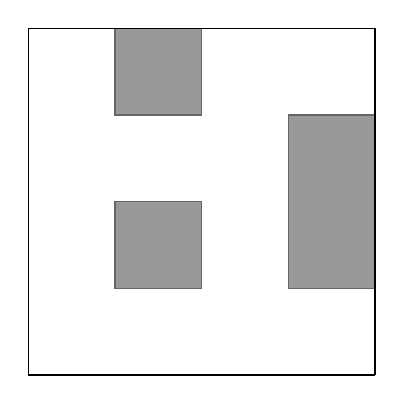
\begin{tikzpicture}[scale=1.1,line width=0.5pt]
      
      \filldraw[color=black!60,fill=black!40] (1,1) rectangle (2,2); 
      \filldraw[color=black!60,fill=black!40] (1,3) rectangle (2,4); 
      \filldraw[color=black!60,fill=black!40] (3,1) rectangle (4,3); 
      %\draw[color=black!60] (0,0) grid (4,4);
      
      \draw[black] (0,0) -- (4,0);
      \draw[black] (0,0) -- (0,4);
      \draw[black] (4,4) -- (4,0);
      \draw[black] (4,4) -- (0,4);
     
    \end{tikzpicture}
  \caption{A map of size $4^{2}$}
  %\label{fig:fig}
\end{figure}

\begin{description}
\item{\bfseries Valid location}\\
The agent is modelled as a dimensionless point, as is the convention\cite{Daniel10} \todo{is this the correct way to reference it?} in any-angle pathfinding research. Therefore, a valid location is defined as any location $(x,y) \in M$ that lies in a free cell or on the boundary of a free cell.
\end{description}

\begin{description}
\item{\bfseries Line of sight}\\
A line of sight exists between two locations $(x_{0},y_{0})$ and $(x_{1},y_{1})$ on a map if all locations that lie on the straight line drawn between $(x_{0},y_{0})$ and $(x_{1},y_{1})$ are valid --- that is to say, for all $t \in \mathbb{R}$ where $0 \leq t \leq 1$: $(x_{0} + t(x_{1}-x_{0}),y_{0} + t(y_{1}-y_{0}))$ is a valid location. The existence of a line of sight between two locations implies that an agent can travel in a straight line between the two locations.
\end{description}

\begin{description}
\item{\bfseries Path through a map}\\
A path  $P_{M} = ((x_{0},y_{0}), (x_{1},y_{1}), \ldots, (x_{n},y_{n}))$ through map $M$ is an ordered list of coordinates $(x,y) \in M$ where $(x_{0},y_{0})$ = $(x_{start},y_{start})$ is the $start$ location of the path, and $(x_{n},y_{n})$ = $(x_{goal},y_{goal})$ is the $goal$ location of the path. A path is valid if there exists a line of sight between every pair of coordinates that are adjacent in the path: $(x_{i},y_{i})$ and $(x_{i+1},y_{i+1})$.

\noindent
It should be noted that since the agent is modelled as a dimensionless point, the path through the map shown in Figure 2.2, which features a `diagonal blockage', is a valid path.\\

\end{description}

\begin{figure}[h]
    \centering
    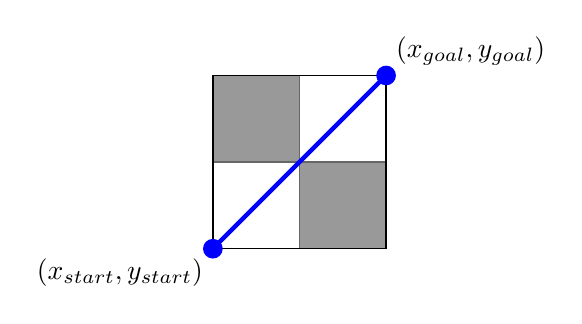
\begin{tikzpicture}[scale=1.1,line width=0.5pt]
    
      \draw[black!60] (0,0) grid (2,2);
      \filldraw[color=black!60,fill=black!40] (0,1) rectangle (1,2); 
      \filldraw[color=black!60,fill=black!40] (1,0) rectangle (2,1); 
      \draw (0,0) -- (2,0);
      \draw (0,0) -- (0,2);
      \draw (2,2) -- (2,0);
      \draw (2,2) -- (0,2);
      \node[below left] at (0,0) {$(x_{start},y_{start})$};
      \node[above right] at (2,2) {$(x_{goal},y_{goal})$};
      \filldraw[blue] (0,0) circle (3pt);
      \filldraw[blue] (2,2) circle (3pt);
      \draw[blue, ultra thick] (0,0) -- (2,2);
      
          
    \end{tikzpicture}
  \caption{A valid path for an agent modelled as a point}
  %\label{fig:fig}
\end{figure}

\subsection{Graph}

Pathfinding algorithms operate on graphs. Therefore, to find an optimal or near-optimal path through a map between a given $start$ and $goal$, the following steps are taken:
\begin{enumerate}
\item a graph that represents the map is produced, where each node in the graph represents a location in the map; 
\item a pathfinding algorithm is applied to the graph, which returns a path through the graph;
\item this path through the graph corresponds to a path through the map.
\end{enumerate}
Step 1 is introduced in the upcoming {\bfseries Discretisation} subsection. Step 2 is introduced in section {\bfseries 2.2: Any-angle pathfinding algorithms}. Step 3 is a result of the definition of a graph, which now follows:\\

\noindent
{\bfseries Graph}\\
\noindent
A graph $G_{M}=(V,E)$ is a representation, or abstraction, of a map $M$. Each node $n \in V$ represents a valid location $(a,b) \in M$. If there is a line of sight between two locations in $M$ then the the two nodes $n$ and $n'$ that represent these locations are connected by an edge $e=(n,n') \in E$, and are thus called `neighbours'. $(n,n').weight$ is the distance an agent would traverse by travelling directly between the two locations i.e. the Euclidean distance between those locations.

\begin{description}
\item{\bfseries Path through a graph}\\
A path $P_{G_{M}} = (n_{0}, n_{1}, \ldots, n_{n})$ through graph $G_{M}=(V,E)$ is a list of nodes $n \in V$, where $n_{0}=n_{start}$ and $n_{n}=n_{goal}$. A path is valid if, for each pair of nodes $n_{i}$ and $n_{i+1}$, there exists an edge $(n_{i},n_{i+1}) \in E$.
\end{description}

\noindent
{\bfseries Lattice}\\
\noindent
The concept of a lattice $L_{N}$ is introduced because lattices will be used in the next subsection, {\bfseries Discretisation}, to conceptually explain how a graph is created such that it represents a specific map. A lattice is a graph of $N^{2}$ nodes where $N \in\mathbb{Z}$ and $N > 0$, and can be thought of as a graph that represents a map with no blocked cells. There are two types of lattice:\\

\begin{description}
\item{\bfseries Octile lattice $L_{N,O}$}\\The nodes of the lattice are arranged in a square grid, and each node is connected by an edge to the closest node, if any exists, at a bearing of any integer multiple of $\frac{\pi}{4}$ radians. See Figure 2.3 (a).

\item{\bfseries Full lattice $L_{N,F}$}\\The nodes of the lattice are arranged in a square grid, and each node is connected by an edge to every other node in the lattice. See Figure 2.3 (b).
\end{description}

\begin{figure}[h]
  \begin{subfigure}{.5\textwidth}
    \centering
    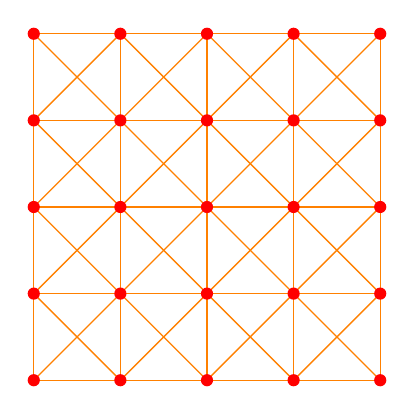
\begin{tikzpicture}[scale=1.1,line width=0.5pt]
      
      \draw[orange] (0,0) grid (4,4);
  
      \foreach \x in {0,1,2,3} {
        \foreach \y in {0,1,2,3} {
          \pgfmathparse{int(\x + 1)};
          \let\xa\pgfmathresult;
          \pgfmathparse{int(\y + 1)};
          \let\ya\pgfmathresult;
          \draw[orange] (\x,\y) -- (\xa,\ya);
        }
      }
  
      \foreach \x in {0,1,2,3} {
        \foreach \y in {1,2,3,4} {
          \pgfmathparse{int(\x + 1)};
          \let\xa\pgfmathresult;
          \pgfmathparse{int(\y - 1)};
          \let\ya\pgfmathresult;
          \draw[orange] (\x,\y) -- (\xa,\ya);
        }
      }
      
      \foreach \x in {0,1,2,3,4} {
        \foreach \y in {0,1,2,3,4} {
          \fill[red] (\x,\y) circle (2pt);
        }
      }
     
    \end{tikzpicture}
    \caption[Map]{Octile lattice $L_{N,O}$}
    %\label{fig:sfig1}
  \end{subfigure}
  %
  \begin{subfigure}{.5\textwidth}
    \centering
    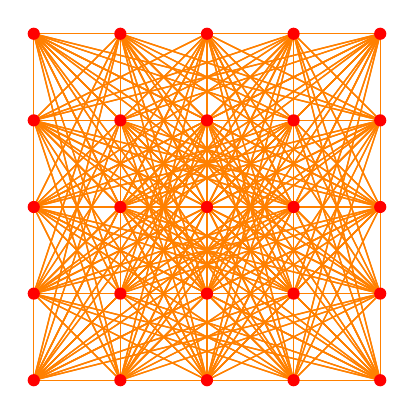
\begin{tikzpicture}[scale=1.1,line width=0.5pt]
      
      \draw[orange] (0,0) grid (4,4);
      
       \foreach \x in {0,1,2,3,4} {
        \foreach \y in {0,1,2,3,4} {
          \foreach \a in {0,1,2,3,4} {
            \foreach \b in {0,1,2,3,4} {
              \draw[orange] (\x,\y) -- (\a,\b);
            }
          }
        }
      }
      
            \foreach \x in {0,1,2,3,4} {
        \foreach \y in {0,1,2,3,4} {
          \fill[red] (\x,\y) circle (2pt);
        }
      }

    \end{tikzpicture}
    \caption{Full lattice $L_{N,F}$}
    %\label{fig:sfi2}
  \end{subfigure}
  \caption{Octile lattice and full lattice of size $4^{2}$}
  %\label{fig:fig}
\end{figure}

\noindent
{\bfseries Discretisation}\\
\noindent
Discretisation is the process of creating a graph $G_{M}=(V,E)$ that represents a map $M$. The process can be visualised as refining a lattice by removing edges and nodes until the desired graph remains. A node $n$ is removed if the map indicates that $n$ represents an invalid location, and an edge $(n,n')$ is removed if there is no line of sight on the map between the locations represented by $n$ and $n'$. Two different types of graphs are produced, depending on whether the original lattice is an octile lattice or a full lattice.\\

\begin{description}
\item{\bfseries Grid-based graph: $d_{G}(L_{O},M) \rightarrow G_{M,G}$}\\
A grid-based graph $G_{M,G}$ has a node to represent every valid location that lies on a corner of a cell in $M$. Each node is connected to each of the up to eight nodes that directly surround it\footnote{If node $n$ represents location $(i,j)$, the ``up to eight nodes that directly surround it'' are the nodes that represent the locations $(i-1,j-1)$, $(i-1,j)$, $(i-1,j+1)$, $(i,j+1)$, $(i+1,j+1)$, $(i+1,j)$, $(i+1,j-1)$ and $(i-1,j)$.} if there is a line of sight between those two nodes. A formal description of the discretisation process that creates a grid-based graph is now provided:\\

An octile lattice $L_{N,O}$ is laid over $M$ such that each node in $L_{N,O}$ lies directly on top of a coordinate $(x,y)$ in $M$. If none of the (up to) four cells surrounding a node\footnote{In a map $M$ of size $N^{2}$, the ``four cells surrounding'' a node that represents coordinate $(a,b) \in M$ are the cells $(a,b)$, $(a,b-1)$, $(a-1,b-1)$ and $(a-1,b)$ if they exist, where $0 \leq a,b \leq N$.} are free then that node is removed, along with all edges that are connected to it. Additionally, if a cell is blocked, diagonal edges that cross that cell are removed, along with any horizontal or vertical edges that lie beneath the blocked cell and are also on the boundary of the lattice.

\item{\bfseries Visibility graph: $d_{V}(L_{O},M) \rightarrow G_{M,V}$}\\
A visibility graph is created so that the optimal path through it is guaranteed to correspond to the shortest path through the map that it represents, whereas the shortest path through a grid-based graph may not\cite{Nash11} have this property. To achieve this, a visibility graph $G_{M,V}$ has a node to represent the $start$ and $end$ locations of the desired path, and node to represent every location that could conceivably lie on a shortest path. It can be shown\cite{Nash11} that any location that does not lie on the corner of a cell where exactly three of the four surrounding cells are blocked cannot conceivably lie on a shortest path. Each node is connected to any node to which it has a line of sight, as implied by the name `visibility graph'. A formal description of the discretisation process that creates a visibility graph is now provided:\\

A full lattice $L_{N,O}$ is laid over $M$ such that each node in $L_{N,O}$ lies directly on top of a coordinate $(x,y)$ in $M$. Unless {\em either} exactly three of the (up to) four cells surrounding a node are free {\em or} the node is $n_{start}$ or $n_{goal}$ then that node is removed, along with all edges that are connected to it --- since such nodes are guaranteed to not be on the shortest path. In addition each edge $(n,n') \in E$ is removed if there is no line of sight between the locations that $n$ and $n'$ represent.\\

\end{description}

\begin{figure}[h]
  \begin{subfigure}{.5\textwidth}
    \centering
    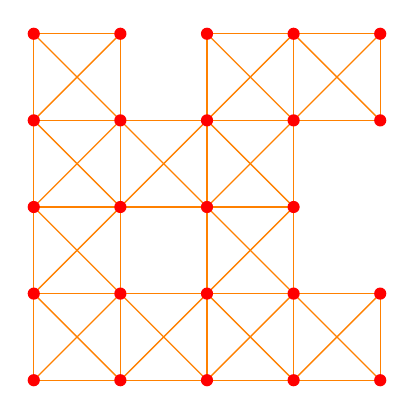
\begin{tikzpicture}[scale=1.1,line width=0.5pt]
      
      \draw[orange] (0,0) grid (4,4);
  
      \foreach \x in {0,1,2,3} {
        \foreach \y in {0,1,2,3} {
          \pgfmathparse{int(\x + 1)};
          \let\xa\pgfmathresult;
          \pgfmathparse{int(\y + 1)};
          \let\ya\pgfmathresult;
          \draw[orange] (\x,\y) -- (\xa,\ya);
        }
      }
  
      \foreach \x in {0,1,2,3} {
        \foreach \y in {1,2,3,4} {
          \pgfmathparse{int(\x + 1)};
          \let\xa\pgfmathresult;
          \pgfmathparse{int(\y - 1)};
          \let\ya\pgfmathresult;
          \draw[orange] (\x,\y) -- (\xa,\ya);
        }
      }
      
      \filldraw[color=orange,fill=white] (1,1) rectangle (2,2);
      \filldraw[color=orange,fill=white] (1,3) rectangle (2,4);
      \draw[white, ultra thick] (1,4) -- (2,4);
      \filldraw[color=orange,fill=white] (3,1) rectangle (4,3);
      \draw[white, ultra thick] (4,1) -- (4,3);
      
      \foreach \x in {0,1,2,3} {
        \foreach \y in {0,1,2,3,4} {
          \fill[red] (\x,\y) circle (2pt);
        }
      }
      \fill[red] (4,0) circle (2pt);
      \fill[red] (4,1) circle (2pt);
      \fill[red] (4,3) circle (2pt);
      \fill[red] (4,4) circle (2pt);
     
    \end{tikzpicture}
    \caption[Map]{Grid-based graph $G_{M,G}$}
    %\label{fig:sfig1}
  \end{subfigure}
  %
  \begin{subfigure}{.5\textwidth}
    \centering
    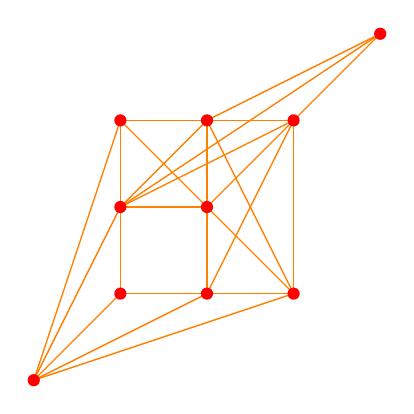
\begin{tikzpicture}[scale=1.1,line width=0.5pt]

     \draw[orange] (0,0) -- (1,1);
     \draw[orange] (0,0) -- (1,2);
     \draw[orange] (0,0) -- (1,3);
     \draw[orange] (0,0) -- (2,1);
     \draw[orange] (0,0) -- (3,1);
     
     \draw[orange] (1,1) -- (1,3);
     \draw[orange] (1,1) -- (3,1);
     
     \draw[orange] (1,2) -- (2,2);
     \draw[orange] (1,2) -- (2,3);
     \draw[orange] (1,2) -- (3,3);
     \draw[orange] (1,2) -- (4,4);
     
     \draw[orange] (1,3) -- (3,3);
     \draw[orange] (1,3) -- (3,1);
     
     \draw[orange] (2,1) -- (2,3);
     \draw[orange] (2,1) -- (3,3);
     
     \draw[orange] (2,2) -- (4,4);
     
     \draw[orange] (3,1) -- (3,3);
     \draw[orange] (3,1) -- (2,3);
     
     \draw[orange] (2,3) -- (4,4);
     
     \fill[red] (0,0) circle (2pt);
     \fill[red] (1,1) circle (2pt);
     \fill[red] (1,2) circle (2pt);
     \fill[red] (1,3) circle (2pt);
     \fill[red] (2,1) circle (2pt);
     \fill[red] (2,2) circle (2pt);
     \fill[red] (2,3) circle (2pt);
     \fill[red] (3,1) circle (2pt);
     \fill[red] (3,3) circle (2pt);
     \fill[red] (4,4) circle (2pt);
     

    \end{tikzpicture}
    \caption{Visibility graph $G_{M,V}$}
    %\label{fig:sfi2}
  \end{subfigure}
  \caption[Graph representations of map $M$]{Graph representations of map $M$, where $n_{start} = (0,0)$ and $n_{goal} = (4,4)$}
  %\label{fig:fig}
\end{figure}

\subsection{The any-angle pathfinding problem}

The problem is to compute optimal or near-optimal paths, if they exist, between a given $start$ and $goal$ location in a map, by using a grid-based graph\footnote{The optimal path through a visibility graph is guaranteed to correspond to the optimal path through the map that it represents, whereas the optimal path through a grid-based graph may not\cite{Nash11}. However, grid-based graphs are generally accepted as the preferable form of map representation for pathfinding since, for a map $M$ of size $N^{2}$, a grid-based graph has {$O(N^{2})$} edges, whereas a visibility graph has {$O(N^{4})$} edges. Therefore for large maps, grid-based graphs are a far more space-efficient representation than visibility graphs. For this reason, this investigation will focus predominantly on pathfinding algorithms applied to grid-based graphs.}.\\

\noindent
An path $P_{M}$ through map $M$ is optimal, denoted as $P^{*}_{M}$, if there do not exist any paths through $M$ from $start$ to $goal$ with a shorter path length and a smaller path angle-sum, where:

\begin{description}
\item{\bfseries Path length}\\
The sum of the Euclidean distances between each pair of coordinates $(x_{i},y_{i})$ and $(x_{i+1},y_{i+1})$ in $P_{M}$.
\item{\bfseries Path angle-sum}\\
The sum of the (smaller) angles between each pair of path segments $(x_{i},y_{i})$ to $(x_{i+1},y_{i+1})$ and $(x_{i+1},y_{i+1})$ to $(x_{i+2},y_{i+2})$ in $P_{M}$. This is given by the scalar product between the two path segments. See figure 2.5.
\end{description}

\begin{figure}
   \centering
    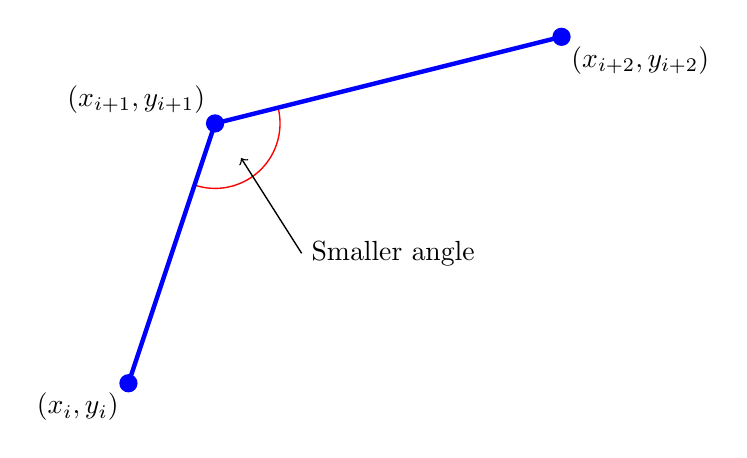
\begin{tikzpicture}[scale=1.1,line width=0.5pt]
      
     \fill[blue] (0,0) circle (3pt);
     \node[below left] at (0,0) {$(x_{i},y_{i})$};
     \fill[blue] (1,3) circle (3pt);
     \node[above left] at (1,3) {$(x_{i+1},y_{i+1})$};
     \fill[blue] (5,4) circle (3pt);
     \node[below right] at (5,4) {$(x_{i+2},y_{i+2})$};
     
     \draw[red] (1,3) ++(-108.4:0.75) arc (-108.41:14:0.75);
     %\draw[red] (1,3) circle (0.75);
     
     \draw[blue,ultra thick] (0,0) -- (1,3) -- (5,4);
     
     \node[right] at (2,1.5) {Smaller angle};
     \draw[->] (2,1.5) -- (1.3,2.6);
     
    \end{tikzpicture}
    \caption{Smaller angle between a pair of path segments}
    %\label{fig:sfig1}
  \end{figure}


\subsection{Solving the any-angle pathfinding problem}

\noindent
The steps required to find an optimal or near-optimal path $P_{M}$ through a map $M$ from $start$ to $goal$, as introduced in subsection {\bfseries 2.1.2: Graph}, will now be re-stated using the notation that has been introduced in this chapter:
\begin{enumerate}
\item a graph $G_{M}$ that represents the map $M$ is produced, where each node in the graph represents a location in the map; 
\item a pathfinding algorithm\footnote{{\em Block A*} operates in a different way, and will be dealt with separately.} is applied to the $G_{M}$, which returns a path $P_{G_{M}} = (n_{start},n_{1},...,n_{goal})$;
\item $P_{G_{M}}$ corresponds to the path $P_{M} = (x_{start},x_{1},...,x_{goal})$, using the correspondence that $x_{i}$ is the location in map $M$ that is represented by the node $n_{i}$ of graph $G_{M}$.
\end{enumerate}

\noindent
The only step that remains to be introduced is step 2 which involves the application of a pathfinding algorithm to a graph. This topic is covered thoroughly in the following section.

\section{Any-angle pathfinding algorithms}

\noindent
This section starts with an introduction of pathfinding over graphs, followed by definitions of the two types of pathfinding algorithms: `classic' and 'any-angle'. The remainder of the section describes two classic pathfinding algorithms: {\em Dijktra's shortest paths}\cite{Dij59} and {\em A*}\cite{Hart68}, followed by the four any-angle pathfinding algorithms that form the core investigation in this dissertation: {\em A* with post smoothing}, {\em Theta*}, {\em Lazy Theta*} and {\em Block A*}.

\subsection{Pathfinding over graphs}

When applied to a graph $G_{M}$, a pathfinding algorithm returns a path $P_{G{M}}$ between a given $n_{start}$ and $n_{goal}$.\\

\noindent
Section {\bfseries 2.1.3: Graphs} introduced the concept of a graph $G_{M}$ that is a representation of a map $M$. Each node $n$ in $G_{M}$ has an associated coordinate $coord$, and a set of parameters whose values change during the execution of the pathfinding algorithm. Some of the parameters may be different for different algorithms, though all of the algorithms use the following two parameters:
\begin{itemize}
\item {\em g-value} --- the path length of the shortest path between $n_{start}$ and $n$ that the algorithm has found thus far;
\item {\em parent} --- a pointer to the previous node in the shortest path between $n_{start}$ and $n$ that the algorithm has found thus far. Therefore, the shortest path between $n_{start}$ and $n$ is found by recursively following the $parent$ pointers from $n$ to $n_{start}$.
\end{itemize}

\noindent
When the algorithm is initialised, $n.g = \infty$ and $n.parent = \bot$\footnote{Where $\bot$ denotes that the parameter value is undefined.} for all nodes, since the algorithm hasn't found any paths between any nodes at this point.\\

\noindent
From the definitions of $g-value$ and the $parent$ pointers, it can be seen that when the algorithm terminates: $n_{goal}.g$ is the path length of the shortest path (if one exists) found by the algorithm from $n_{start}$ to $n_{goal}$, and the shortest path (if one exists) can be found by recursively following the $parent$ pointers from $n_{goal}$ to $n_{start}$\footnote{The pathfinding algorithm guarantees $n_{start}.parent = \bot$.}.

\subsection {Types of pathfinding algorithms}

A summary of our findings so far motivates the need for a more advanced type of pathfinding algorithm than the classic pathfinding algorithms:\\

\noindent
As seen in the {\bfseries Introduction}, even though a path through a grid-based graph $G_{M,G}$ may be optimal, the corresponding path through the $M$ may not be optimal. Furthermore, subsection {\bfseries 2.1.2: Graph} introduced the fact that an when an optimal path is found through a visibility graph $G_{M,V}$, the corresponding path through $M$ is guaranteed to be optimal. Since classic pathfinding algorithms find optimal paths through graphs, and because the decision has been made to use grid-based graphs over visibility graphs (since visibility graphs tend to be very large, and therefore expensive to store and traverse), it is clear that using classic pathfinding algorithms will give sub-optimal paths through maps.\\

\noindent
Any-angle pathfinding algorithms aim to improve upon classic pathfinding algorithms by taking a grid-base graph $G_{M,G}$ and selectively adding a small amount of edges to $G_{M,G}$ (i.e. `augmenting' $G_{M,G}$) so that it closely resembles a visibility graph in the region that surrounds the path. In this way, any-angle pathfinding algorithms aim to benefit from the efficiency of grid-based graphs and the optimality of visibility graphs, though tradeoffs are required on both sides. These explanations are now formalised:

\begin{description}
\item{\bfseries Classic pathfinding algorithm}\\ 
A classic pathfinding algorithm will return the optimal\footnote{The definition of an optimal path $P_{G_{M}}$ through a graph is analogous to the definition of a an optimal path $P_{M}$ in subsection {\bfseries 2.1.3: The any-angle pathfinding problem}.}  path $P^{*}_{G_{M}}$ through $G_{M}$\footnote{Remember: $P_{G_{M}}$ corresponds to $P_{M}$, but the optimal path $P^{*}_{G_{M}}$ through $G_{M}$ does not necessarily correspond to the optimal path $P^{*}_{M}$ through $M$ --- this idea was illustrated in the {\bfseries Introduction} chapter.}.
\item{\bfseries Any-angle pathfinding algorithm}\\
An any-angle pathfinding algorithm will return the optimal path $P^{*}_{G'_{M}}$ through $G'_{M}$, where the augmented graph $G'_{M}$ may have extra edges to $G_{M}$.
\end{description}

\noindent
This dissertation focuses on any-angle pathfinding algorithms, but two classic pathfinding algorithms {\em Dijkstra's shortest paths} and {\em A*} are presented first as they explain some of the important concepts required to understand the more complicated any-angle algorithms, and to serve as a useful benchmark for comparison in the {\bfseries Evaluation} chapter.

\subsection {Dijkstra's shortest paths}

Most of the algorithms in this dissertation are derivatives of the {\em A*} graph traversal algorithm, which itself is a derivative of {\em Dijkstra}'s famous shortest-path algorithm.\\

\noindent
{\bf Overview}\\
\noindent
{\em Dijkstra's shortest paths} is a classic pathfinding algorithm, which finds an optimal path\cite{Dij59} $P^{*}_{G}$ through a graph $G$. Starting at $n_{start}$, {\em Dijkstra} selects and then processes (or `expands') one node at a time (see subsection {\bfseries Expansion}). It is a provable\cite{CormenDijkstra} invariant of the algorithm that when a node $n$ is selected to be processed, $n.g$ is equal to the length of the shortest path in the graph to $n$ from $n_{start}$. For this reason, once a node has been expanded, it need not be expanded again (this would incur unnecessary work) --- a set $closedSet$\footnote{The set and priority queue methods $add()$, $pop()$ and  $contains()$ are defined in the usual way.} ensures that this does not occur. When $n_{goal}$ is expanded, $n_{goal}.g$ is the length of the shortest path in $G_{M}$ from $n_{start}$ to $n_{goal}$ (according to the invariant condition), so the algorithm terminates.\\

\noindent
{\bf Expansion}\\
\noindent
{\em Dijkstra} selects the next node $n$ to expand from $openSet$, a priority queue that stores nodes in increasing order of their {\em g-values}. To expand $n$: for each $n_{neigh}$ of the neighbours of $n$, {\em Dijkstra} attempts to `relax' $n_{neigh}$ --- that is to say: {\em Dijkstra} tests whether the shortest path to $n_{neigh}$ that it had found so far (as defined by the $parent$ pointers from $n$ to $n_{start}$) is longer than the path to $n_{neigh}$ that is made up of the shortest path found so far to $n$ and then from $n$ to $n_{neigh}$\footnote{This condition relies on the provable\cite{CormenDijkstra} fact that any sub-path of a shortest path is itself a shortest path.}, which can be stated as the condition:
\begin{equation}
n.g + (n,n_{neigh}).weight < n_{neigh}.g
\end{equation}
\noindent
and if (2.1) is true, {\em Dijkstra} updates $n_{neigh}$ to reflect that the newly discovered shortest path to it is the one that goes via $n$, by: 
\begin{itemize}
\item updating the $parent$ of $n_{neigh}$ to $n$;
\item updating the {\em g-value} of $n_{neigh}$ to $n.g + (n,n_{neigh}).weight$ .
\end{itemize}
Finally, $n_{neigh}$ is added to $openSet$ if it is not already in it, and then the next node to be expanded is selected.\\

\noindent
{\bf Termination}\\
\noindent
This process continues until $openSet$ is empty or $n_{goal}$ has been processed, at which point the algorithm terminates. If a valid path exists, {\em Dijkstra} returns $P^{*}_{G}$. Otherwise it returns $\bot$.\

\begin{algorithm}
  \SetAlgoLined\DontPrintSemicolon
  \SetKwFunction{dijkstra}{Dijkstra}\SetKwFunction{update}{Update}
  \SetKwProg{myDef}{def}{}{}
  \myDef{\dijkstra{G, $n_{start}$, $n_{goal}$}}{
  \nl $openSet \gets \bot$\;
  \nl $closedSet \gets \bot$\;
  \nl $n_{start}.g \gets 0$\;
  \nl $openSet.add(n_{start})$\;
  \nl \While{$openSet \neq \bot$} {
    \nl $n_{curr} \gets openSet.pop()$\;
    \nl $closedSet.add(n_{curr})$\;
    \nl \If{$n_{curr} = n_{goal}$} {
      \nl \KwRet{$n_{goal}$}\;
    }
    \nl \ForEach{$n_{neigh}$ of $n_{curr} $} {
      \nl \If{$closedSet.contains(n_{neigh}) = false $} {
        \nl \If{$\update(n_{neigh}) = true$} {
          \nl \If{$openSet.contains(n_{neigh}) = false $} {
            \nl $openSet.add(n_{neigh})$\;
          }
        }
      }
    }
  }
  \nl \KwRet{$\bot$}\;
}{}
  \setcounter{AlgoLine}{0}
  \myDef{\update{$n_{neigh}$}}{
    \nl \uIf{$n_{curr}.g + (n_{curr},n_{neigh}).weight < n_{neigh}.g$} {
      \nl $n_{neigh}.g = n_{curr}.g + (n_{curr},n_{neigh}).weight$\;
      \nl $n_{neigh}.parent = n_{curr}$\;
      \nl \KwRet{$true$}\;
    } \nl \Else {
      \nl \KwRet{$false$}\;
    } 
  }
  \caption{{\sc Dijkstra}}
\end{algorithm} 

\subsection {A*}

{\em A*} is based on {\em Dijkstra's shortest-paths} algorithm and finds the optimal path\cite{Hart68} $P^{*}_{G}$ through a graph $G$, but uses a heuristic $h$ to reduce the number of node expansions.\\

\noindent
In addition to a {\em g-value} and a {\em parent}, each node also has a\todo{Arbitrary choice between node having h-value or f-value?}:
\begin{itemize}
\item {\em h-value} --- Euclidean distance between {$n$} and {$n_{goal}$}: a cheaply computable monotonic estimate\footnote{The monotonicity of Euclidean distance as a heuristic ensures that {\em A*}, like {\em Dijkstra}, is complete (if a path exists, it finds it) and optimal (if a path is found, it is a shortest distance path)} of the actual shortest path length between $n$ and $n_{goal}$.
\end{itemize}

\noindent
While {\em Dijkstra} preferentially expands nodes with low {\em g-value}s (by utilising a priority queue called {\em openSet}, which sorts using {\em g-values}), {\em A*} preferentially expands nodes with low {\em f-score}s (by utilising a priority queue called {\em openSet}, which sorts using {\em f-values}), where a node $n$'s {\em f-score} is the algorithm's current estimate of the shortest path from $n_{start}$ via $n$ to $n_{goal}$ --- that is to say:
\begin{equation}
n.f = n.g + n.h
\end{equation}

\noindent
The pseudocode for {\em A*} differs only from {\em Dijkstra} in the {\tt Update} subroutine, where the {\em h-score} must also be set.

\begin{algorithm}
  \SetAlgoLined\DontPrintSemicolon
  \SetKwFunction{update}{Update}
  \SetKwProg{myDef}{def}{}{}
  \myDef{\update{$n_{neigh}$}}{
    \nl \uIf{$n_{curr}.g + (n_{curr},n_{neigh}).weight < n_{neigh}.g$} {
      \nl $n_{neigh}.g \gets n_{curr}.g + euclidean(n_{curr},n_{neigh})$\;
      \nl $n_{neigh}.h \gets euclidean(n_{neigh},n_{goal})$\;
      \nl $n_{neigh}.parent = n_{curr}$\;
      \nl \KwRet{$true$}\;
    } \nl \Else {
      \nl \KwRet{$false$}\;
    } 
  }
  \caption{{\tt Update} from {\sc A*}}
\end{algorithm} 

\subsection {A* with post-smoothing}

{\em A* with post-smoothing} is the first any-angle pathfinding algorithm that is introduced in this project. It uses {\em A*} to find the optimal path through $G_{M}$, denoted by $P*_{G_{M}} = (n_{start}, n_{1}, \ldots, n_{goal})$, which is an approximation to an optimal path through map $M$. It then applies a post-processing step which `smoothes' this path by changing the $parent$ pointer for some nodes in the path --- for example, the $parent$ of a node $n_{j} \in P*_{G_{M}}$ is defined as $n_{j-1}$, but {\em A* with post-smoothing} can smoothe a corner in this path by changing the $parent$ of  $n$ to be a node that is nearer to the $start$ of the path that $n_{j-1}$, i.e. change the parent of $n_{j}$ from $n_{j-1}$ to $n_{i}$, where $i<j-1$. If $G_{M}$ does have an edge between $n{j}$ and $n_{i}$, then this re-parenting procedure has the effecting of adding an edge to $G_{M}$.\todo{Mention that the paths produced are not optimal in $M$?}\\

\noindent
{\bf Algorithm}\\
\noindent
On each iteration, the algorithm considers a node $n_{curr}$. Starting with $n_{curr} = n_{goal}$ a line of sight test is performed from the location represented by $n_{curr}$ to the location represented by $n_{curr}.parent.parent$. If a line of sight exists, $n_{curr}.parent$ is set to $n_{curr}.parent.parent$ --- this has the effect of adding an edge $(n_{curr},n_{curr}.parent.parent)$ to $G$. This process is repeated on $n_{curr}$ until a line of sight test fails, at which point $n_{curr}$ is set to $n_{curr}.parent.parent$\footnote{Note: $n_{curr}.parent.parent$ is the node on which the line of sight test failed.}, and the next iteration commences. See figure 2.5. \\

\noindent
{\bf Termination}\\
\noindent
When $n = n_{start}$, the algorithm terminates.\\

\begin{figure}[h]
  \begin{subfigure}{.3\textwidth}
    \centering
    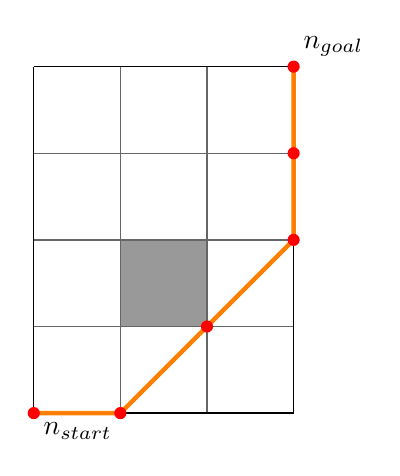
\begin{tikzpicture}[scale=1.1,line width=0.5pt]
    
      \draw[color=black!60] (0,0) grid (3,4);
    
      \node[below right] at (0,0) {$n_{start}$};
      \node[above right] at (3,4) {$n_{goal}$};

      \filldraw[color=black!60,fill=black!40] (1,1) rectangle (2,2); 
      \draw (0,0) -- (0,4);
      \draw (0,0) -- (3,0);
      \draw (3,4) -- (0,4);
      \draw (3,4) -- (3,0);
    
      \draw[orange, ultra thick] (0,0) -- (1,0) -- (3,2) -- (3,4);
      \fill[red] (0,0) circle (2pt);
      \fill[red] (1,0) circle (2pt);
      \fill[red] (2,1) circle (2pt);
      \fill[red] (3,2) circle (2pt);
      \fill[red] (3,3) circle (2pt);
      \fill[red] (3,4) circle (2pt);

    \end{tikzpicture}
    \caption{Original path}
    %\label{fig:sfi2}
  \end{subfigure}
  \begin{subfigure}{.3\textwidth}
    \centering
    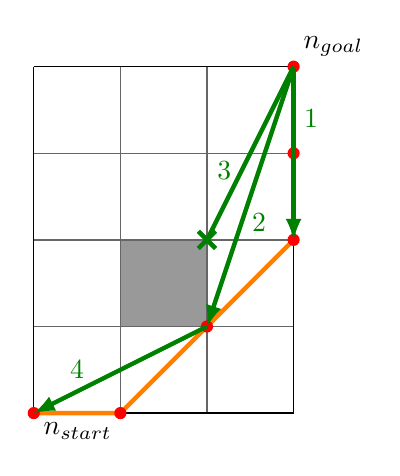
\begin{tikzpicture}[scale=1.1,line width=0.5pt]
    
      \draw[color=black!60] (0,0) grid (3,4);
    
      \node[below right] at (0,0) {$n_{start}$};
      \node[above right] at (3,4) {$n_{goal}$};

      \filldraw[color=black!60,fill=black!40] (1,1) rectangle (2,2); 
      \draw (0,0) -- (0,4);
      \draw (0,0) -- (3,0);
      \draw (3,4) -- (0,4);
      \draw (3,4) -- (3,0);
      
      \draw[orange, ultra thick] (0,0) -- (1,0) -- (3,2) -- (3,4);
      \fill[red] (0,0) circle (2pt);
      \fill[red] (1,0) circle (2pt);
      \fill[red] (2,1) circle (2pt);
      \fill[red] (3,2) circle (2pt);
      \fill[red] (3,3) circle (2pt);
      \fill[red] (3,4) circle (2pt);
      
      \draw[green!50!black, ultra thick,>=latex,->] (3,4) -- (3,2);
      \draw[green!50!black, ultra thick,>=latex,->] (3,4) -- (2,1);
      \draw[green!50!black, ultra thick] (3,4) -- (2,2);
      \draw[green!50!black,ultra thick] (1.9,2.1) -- (2.1,1.9);
      \draw[green!50!black,ultra thick] (1.9,1.9) -- (2.1,2.1);
      \draw[green!50!black, ultra thick, >=latex,->] (2,1) -- (0,0);
      
      \node[green!50!black] at (3.2,3.4) {1};
      \node[green!50!black] at (2.6,2.2) {2};
      \node[green!50!black] at (2.2,2.8) {3};
      \node[green!50!black] at (0.5,0.5) {4};


    \end{tikzpicture}
    \caption{Line of sight tests} \label{fig:astarsmoothed}
  \end{subfigure}
  %
  \begin{subfigure}{.3\textwidth}
    \centering
    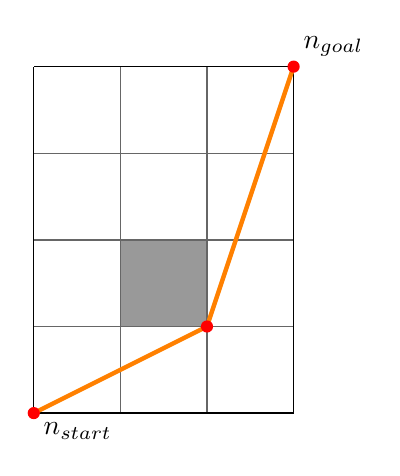
\begin{tikzpicture}[scale=1.1,line width=0.5pt]
    
      \draw[color=black!60] (0,0) grid (3,4);
    
      \node[below right] at (0,0) {$n_{start}$};
      \node[above right] at (3,4) {$n_{goal}$};

      \filldraw[color=black!60,fill=black!40] (1,1) rectangle (2,2); 
      \draw (0,0) -- (0,4);
      \draw (0,0) -- (3,0);
      \draw (3,4) -- (0,4);
      \draw (3,4) -- (3,0);
    
      \draw[orange, ultra thick] (0,0) -- (2,1) -- (3,4);
      \fill[red] (0,0) circle (2pt);
      \fill[red] (2,1) circle (2pt);
      \fill[red] (3,4) circle (2pt);

    \end{tikzpicture}
    \caption{Improved path}
    %\label{fig:sfi2}
  \end{subfigure}
  \caption{A* with post-smoothing}
  %\label{fig:fig}
\end{figure}


\begin{algorithm}
  \SetAlgoLined\DontPrintSemicolon
  \SetKwFunction{ps}{PostSmoothing}\SetKwFunction{los}{LineOfSight}
  \SetKwProg{myDef}{def}{}{}
  \myDef{\ps{$n_{start}, n_{goal}$}}{
    \nl $n_{curr} \gets n_{goal} $\;
    \nl $n_{next} \gets n_{goal}.parent.parent $\;
    \nl \uIf {$n_{next}  = \bot$} {
      \nl \KwRet{} \;
    }
    \nl \While{$true$} {
      \nl \While{$\los(n_{curr} ,n_{next} )$} {
        \nl $n_{curr}.parent \gets n_{next} $\;
        \nl $n_{next}  \gets n_{next} .parent$\;
        \nl \uIf{$n_{next}  = n_{start}$} {
          \nl \KwRet{} \;
        }
      }
      \nl $n_{curr}  \gets n_{next} $\;
      \nl \uIf{$n_{curr}.parent = n_{start}$} {
        \nl \KwRet{}\;
        }
      \nl $n_{next}  \gets n_{next}.parent.parent$\;
    }
  }
  \caption{{\tt PostSmoothing} from {\sc A* with post-smoothing}}
\end{algorithm} 

\subsection {Theta*}

The previous subsection demonstrated how {\em A* with post-smoothing} performs smoothing on the path returned by the classic pathfinding algorithm {\em A*}. In contrast, {\em Theta*} smoothes as it goes along by progressing in a similar way to {\em A*}, but also attempting to re-parent each of $n_{curr}$'s neighbours $n_{neigh}$ with $n_{curr}.parent$ at the time when $n_{curr}$ is expanded\footnote{As with {\em A* with post-smoothing}, re-parenting in {\em Theta*} occurs if a line of sight exists between the coordinates represented by the two nodes in question.}.\\

\noindent
The pseudocode for {\em Theta*} differs only from {\em A*} in the {\tt Update} subroutine. If a line of sight exists between $n_{neigh}.coord$ and $n_{curr}.parent.coord$, {\em Theta*} (notionally) creates an edge $e = (n_{neigh}, n_{curr}.parent)  \in G$ and attempts to relax $e$. However, if the line of sight does not exist $e$ is removed from $G$ and {\em Theta*} mimics {\em A*} by attempting to relax the edge $(n_{neigh},n_{curr})$\footnote{As per the {\tt Update} subroutine of {\em A*}.}.

\begin{algorithm}
  \SetAlgoLined\DontPrintSemicolon
  \SetKwFunction{update}{Update}\SetKwFunction{los}{LineOfSight}
  \SetKwProg{myDef}{def}{}{}
  \myDef{\update{$n_{neigh}$}}{
    \nl \uIf{$\los(n_{neigh}, n_{curr}.parent) = true$} {
      \nl \uIf{$n_{curr}.parent.g + (n_{curr}.parent,n_{neigh}).weight < n_{neigh}.g$} {
        \nl $n_{neigh}.g \gets n_{neigh}.parent.g + (n_{curr}.parent,n_{neigh}).weight$\;
        \nl $n_{neigh}.f \gets euclidean(n_{neigh},n_{goal})$\;
        \nl $n_{neigh}.parent \gets n_{curr}.parent$\;
        \nl \KwRet{$true$}\;
      } \nl \Else {
        \nl \KwRet{$false$}\;
      } 
    } \nl \Else {
      \nl \uIf{$n_{curr}.g + (n_{curr},n_{neigh}).weight < n_{neigh}.g$} {
        \nl $n_{neigh}.g \gets n_{curr}.g + (n_{curr},n_{neigh}).weight$\;
        \nl $n_{neigh}.f \gets euclidean(n_{neigh},n_{goal})$\;
        \nl $n_{neigh}.parent \gets n_{curr}$\;
        \nl \KwRet{$true$}\;
      } \nl \Else {
        \nl \KwRet{$false$}\;
      } 
    }
  }
  \caption{{\tt Update} from {\sc Theta*}}
\end{algorithm} 

\subsection {Lazy Theta*}

{\em Lazy Theta*} attempts to refine {\em Theta*} by finding similar paths despite performing fewer line of sight tests. Where {\em Theta*} performs a line of sight test for every neighbour $n_{neigh}$ of every node $n_{curr}$ that is expanded, {\em Lazy Theta*} only performs line of sight tests for every node $n_{curr}$ that is expanded, since any other tests are redundant. However, because the edge relaxation therefore occurs at a different point of the iteration, the paths returned by {\em Lazy Theta*} are not always the same as those returned by {\em Theta*}.\\

\noindent
The pseudocode for {\em Lazy Theta*} differs from that of {\em Theta*} in the {\tt Expand} subroutine, and also performs an {\tt Initialise} step on each node at the start of each expansion. A more technical explanation of a node expansion in {\em Lazy Theta*} in now presented:\\

\noindent
{\bf Expansion}\\
\noindent
For each $n_{curr}$ that is expanded, {\em Lazy Theta*} assumes that a line of sight exists between $n_{curr}.parent$ and each neighbour $n_{neigh}$ of $n_{curr}$, and updates the {\em g-value} and $parent$ of each $n_{neigh}$ accordingly\footnote{{\em Lazy Theta*} performs the update part of relaxation without first performing the test in equation (2.1)}. {\em Lazy Theta*} only actually performs that line of sight test if the $n_{neigh}$ itself is ever expanded (henceforth referred to as $n_{curr}'$, for clarity), by calling {\tt Initialise} when $n_{curr}'$ is popped off $openSet$. If the line of sight doesn't in fact exist, {\tt Initialise} alters $n_{curr}'$ accordingly\footnote{See {\bfseries Algorithm 5} lines 2-4}.

\begin{algorithm}
  \SetAlgoLined\DontPrintSemicolon
  \SetKwFunction{dijkstra}{LazyTheta*}\SetKwFunction{update}{Update}\SetKwFunction{los}{LineOfSight}\SetKwFunction{init}{Initialise}
  \SetKwProg{myDef}{def}{}{}
  
  \myDef{\dijkstra{G, $n_{start}$, $n_{goal}$}}{
  \nl $openSet \gets \bot$\;
  \nl $closedSet \gets \bot$\;
  \nl $n_{start}.g \gets 0$\;
  \nl $openSet.add(n_{start})$\;
  \nl \While{$openSet \neq \bot$} {
    \nl $n_{curr} \gets openSet.pop()$\;
    \nl $\init(n_{curr})$\;
    \nl $closedSet.add(n_{curr})$\;
    \nl \If{$n_{curr} = n_{goal}$} {
      \nl \KwRet{$n_{goal}$}\;
    }
    \nl \ForEach{$n_{neigh}$ of $n_{curr} $} {
      \nl \If{$closedSet.contains(n_{neigh}) = false $} {
        \nl \If{$\update(n_{neigh}) = true$} {
          \nl \If{$openSet.contains(n_{neigh}) = false $} {
            \nl $openSet.add(n_{neigh})$\;
          }
        }
      }
    }
  }
  \nl \KwRet{$\bot$}\;
}{}

  \myDef{\init{$n_{curr}$}}{
      \nl \uIf{$\los(n_{curr}, n_{curr}.parent) = false$} {
        \nl $newParent \gets \argmin\limits_{n' \in expandedNeigh(n_{curr})} (n'.g + (n',n_{curr}).weight)$\;
        \nl $n_{curr}.parent \gets n'$\;
        \nl $n_{curr}.g \gets n'.g + (n',n_{curr}).weight$\;
       } 
  }
  \myDef{\update{$n_{neigh}$}}{
        \tcp{assume line of sight test passes}
      \nl \uIf{$n_{curr}.parent.g + (n_{curr}.parent,n_{neigh}).weight < n_{neigh}.g$} {
        \nl $n_{neigh}.g \gets n_{neigh}.parent.g + (n_{curr}.parent,n_{neigh}).weight$\;
        \nl $n_{neigh}.f \gets euclidean(n_{neigh},n_{goal})$\;
        \nl $n_{neigh}.parent \gets n_{curr}.parent$\;
        \nl \KwRet{$true$}\;
      } \nl \Else {
        \nl \KwRet{$false$}\;
      } 
  }
  \caption{{\sc Lazy Theta*}}
\end{algorithm} 

\subsection {Block A*}

\noindent
{\em Block A*} is the most complex algorithm in this dissertation. It was published in 2011, and is at the very cutting edge of any-angle path-finding algorithmic research.\\

\noindent
{\bfseries Overview}\\
\noindent
{\em Block A*} aims to achieve faster computation of paths by doing far fewer expansions than the algorithms that have already been introduced, because each expansion in {\em Block A*} processes more than just a single node. As a compromise, each of these expansions is far more complicated than the expansion of a simple node, though this extra complexity is partially assuaged by the use of a {\em Local Distance Database (LDDB)}, which is explained later in this section.\\

\noindent
To elaborate on the brief introduction above: all of the pathfinding algorithms that have already been introduced expand nodes, where the neighbours of the node being expanded may be added to the $openSet$ from which the next node to be expanded is chosen, thus the algorithm makes incremental progress across the graph. The {\em Block A*} algorithm expands `blocks', where a block is a graph-like structure that represents an entire sub-area of the overall map $M$. Therefore, each expansion in {\em Block A*} makes far more progress than an expansion in the other algorithms. The expansion of a block is complicated, as it requires obtaining the values of the shortest paths between points that lie on different sides of a block --- but these do not need to be explicitly calculated because all such paths are available from the {\em LDDB}.\\

\noindent
The remainder of this subsection contains a novel explanation of {\em Block A*} which draws close parallels with the graph-based explanations provided in the previous sections for {\em Dijkstra} and {\em A*}. Due to the complexity of {\em Block A*}, this explanation is mathematically and notationally intensive, yet considerably more succinct that the example based-explanation found in Yap's original paper\cite{Yap11}.\\

\noindent
{\bfseries Blocks}\\
\noindent
A block $B_{i,j}$ of size ${N_{B}}^{2}$ is a graph-like structure that represents the area of the map $M$ covered by all cells $C_{k,l} \in M$ where $i \leq k \leq i+N_{B}$ and $j \leq l \leq j+N_{B}$.\\

\noindent
For each block $B_{i,j} = (V_{i,j},E_{i,j})$, $n \in V_{i,j}$ represents a location $(a,b) \in M$ where $(a,b)$ lies on the boundary of $B_{i,j}$ --- that is to say, where $a=i$ or $a=i+N_{B}$, and $b=j$ or $b=j+N_{B}$. In addition to an associated coordinate, each node $n \in B_{i,j}$ has the parameters:
\begin{itemize}
\item {\em g-value} --- the path length of the shortest path found so far from $n_{start}$ to $n$;
\item {\em h-value} --- Euclidean distance between $n$ and $n_{goal}$\footnote{Except when the block is $B_{goal}$, when the {\em h-value} is the length of the shortest path between $n$ and $n_{goal}$ --- this is discussed in the {\bfseries Initialisation} step.};
\item {\em parent} --- the previous node in the shortest path found so far from $n_{start}$ to $n$.
\end{itemize}

\noindent
Each $block$ $B_{i,j}$ maintains an unordered $openSet_{i,j} \subseteq V_{i,j}$, and a $heapValue_{i,j}$. $openSet_{i,j}$ contains all the nodes in $B_{i,j}$ that have been updated since the block was last expanded --- note that a block can be expanded more than once\footnote{This subtlety caused me such confusion that I eventually emailed Peter Yap, the author of the {\em Block A*} paper, for clarification. He explained the difference, and told me that he had included an explanation of this specific point when he gave a presentation [citation] on Block A* as the confusion is not uncommon.}. $heapValue_{i,j}$ is the smallest {\em f-score} of the nodes in $openSet_{i,j}$\footnote{If $openSet_{i,j} = \bot$, $B_{i,j}.heapValue = \infty$.}, and is used to order blocks in $openSet_{blocks}$, a priority queue that stores blocks in increasing order of their $heapValue$s.\\

\noindent
If the locations represented by $B_{i,j}$ contain the location $start$ or $goal$ then $B_{i,j}$ is called $B_{start}$ or $B_{goal}$ respectively, and $B_{i,j}$ has an extra node $n_{start}$ or $n_{goal}$ with edges from that node to every other node in the block. For all other blocks, called `regular' blocks, there is an edge between every pair of nodes in $B_{i,j}$. See figure 2.7. For all edges $(n,n') \in B$, {\em $(n,n').weight$ is the length of the shortest path in map $M$ between the two locations represented by $n$ and $n'$, and $0 \leq $(n,n').weight$ \leq \infty$}. This important distinction bears clarificiation: in grid-based graphs and visibility graphs, an edge denotes that an agent can travel in a straight line between the two nodes that the edge connects, whereas an edge in a block merely denotes that an agent can travel between those two nodes {\em on some path within that block}, where the length of the shortest path between the two nodes (which may not be a straight line) is the edge weight which may range from $0$ to $\infty$. See figure 2.7\\

\begin{figure}
    \centering
    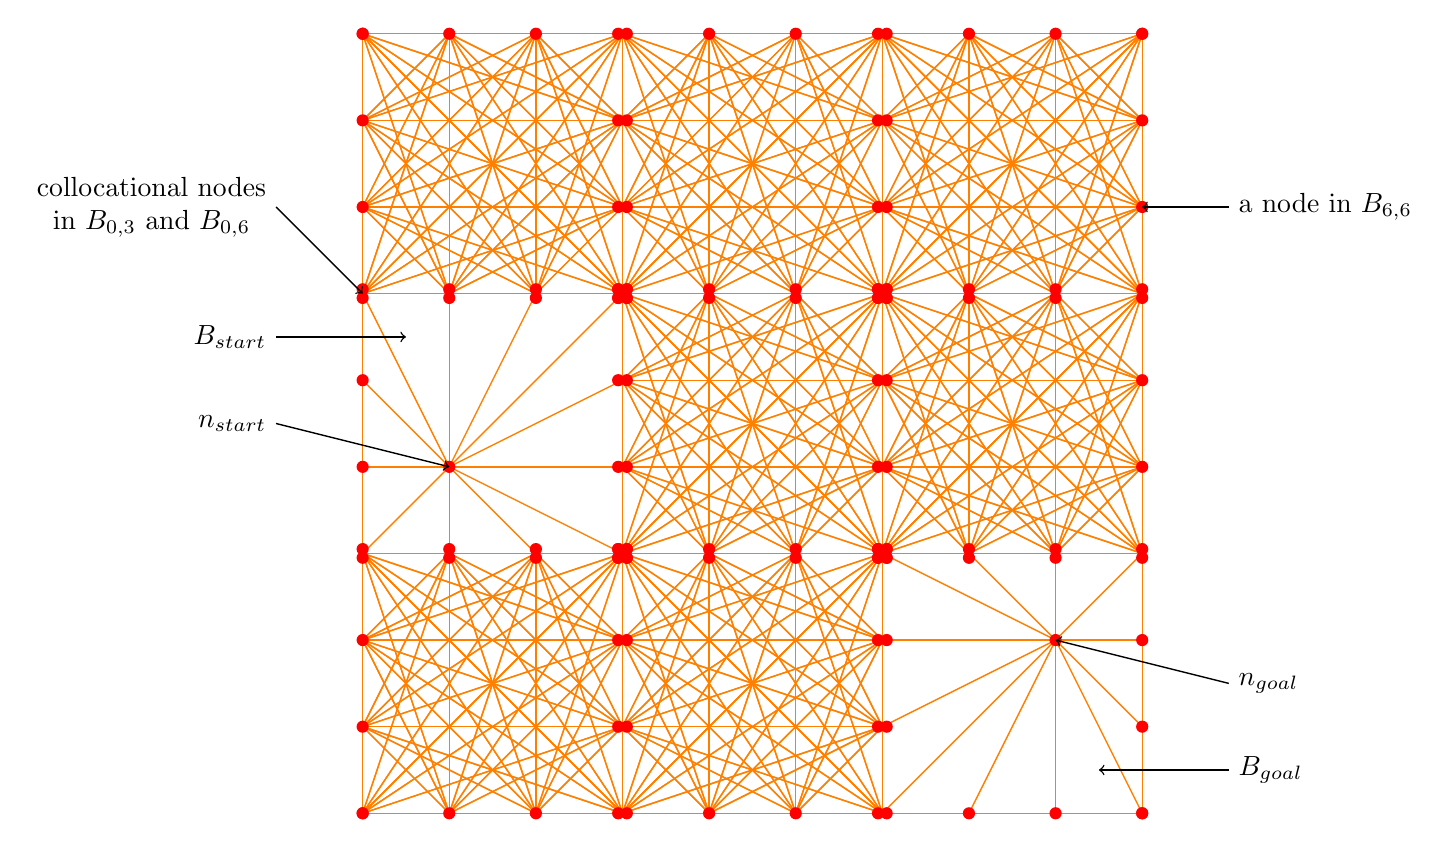
\begin{tikzpicture}[scale=1.1,line width=0.5pt]
  
      \foreach \i in {0,3,6} {
      \foreach \j in {0,3,6} {
      \foreach \x in {0,1,2,3} {
        \foreach \y in {0,3} {
          \foreach \a in {0,1,2,3} {
            \foreach \b in {0,3} {
             \pgfmathparse{int(\x + \i)};
             \let\xn\pgfmathresult;
             \pgfmathparse{int(\a + \i)};
             \let\an\pgfmathresult;
             \pgfmathparse{int(\y + \j)};
             \let\yn\pgfmathresult;
             \pgfmathparse{int(\b + \j)};
             \let\bn\pgfmathresult;
              \draw[orange] (\xn,\yn) -- (\an,\bn);
              \draw[orange] (\yn,\xn) -- (\bn,\an);
            }
          }
        }
      }
      }}
      
      \foreach \i in {0,3,6} {
      \foreach \j in {0,3,6} {
      \foreach \x in {1,2} {
        \foreach \y in {0,3} {
          \foreach \a in {1,2} {
            \foreach \b in {0,3} {
             \pgfmathparse{int(\x+\i)};
             \let\xn\pgfmathresult;
             \pgfmathparse{int(\a+\j)};
             \let\an\pgfmathresult;
             \pgfmathparse{int(\y+\j)};
             \let\yn\pgfmathresult;
             \pgfmathparse{int(\b+\i)};
             \let\bn\pgfmathresult;
              \draw[orange] (\xn,\yn) -- (\bn,\an);
              \draw[orange] (\yn,\xn) -- (\an,\bn);
            }
          }
        }
      }
      }}
      
      \filldraw[color=orange, fill=white] (0,3) rectangle (3,6);
      \filldraw[color=orange, fill=white] (6,0) rectangle (9,3);
      
      \draw[orange] (1,4) -- (0,3);
      \draw[orange] (1,4) -- (0,4);
      \draw[orange] (1,4) -- (0,5);
      \draw[orange] (1,4) -- (0,6);
      \draw[orange] (1,4) -- (3,3);
      \draw[orange] (1,4) -- (3,4);
      \draw[orange] (1,4) -- (3,5);
      \draw[orange] (1,4) -- (3,6);
      \draw[orange] (1,4) -- (1,3);
      \draw[orange] (1,4) -- (2,3);
      \draw[orange] (1,4) -- (1,6);
      \draw[orange] (1,4) -- (2,6);
      \fill[red] (1,4) circle (2pt);
      \draw[orange] (8,2) -- (6,0);
      \draw[orange] (8,2) -- (6,1);
      \draw[orange] (8,2) -- (6,2);
      \draw[orange] (8,2) -- (6,3);
      \draw[orange] (8,2) -- (9,0);
      \draw[orange] (8,2) -- (9,1);
      \draw[orange] (8,2) -- (9,2);
      \draw[orange] (8,2) -- (9,3);
      \draw[orange] (8,2) -- (7,0);
      \draw[orange] (8,2) -- (8,0);
      \draw[orange] (8,2) -- (7,3);
      \draw[orange] (8,2) -- (8,3);
      \fill[red] (8,2) circle (2pt);
      
      \foreach \x in {0,1,2,2.95,3.05,4,5,5.95,6.05,7,8,9} {
        \foreach \y in {0,9} {
              \fill[red] (\x,\y) circle (2pt);
              \fill[red] (\y,\x) circle (2pt);
        }
      }
      
      \foreach \x in {1,2,4,5,7,8} {
        \foreach \y in {3,6} {
          \pgfmathparse{(\y + 0.05)};
           \let\ya\pgfmathresult;
            \pgfmathparse{(\y - 0.05)};
           \let\yb\pgfmathresult;
              \fill[red] (\x,\ya) circle (2pt);
              \fill[red] (\x,\yb) circle (2pt);
              \fill[red] (\ya,\x) circle (2pt);
              \fill[red] (\yb,\x) circle (2pt);
        }
      }
      
       \foreach \x in {3,6} {
        \foreach \y in {3,6} {
          \pgfmathparse{(\x + 0.05)};
           \let\xa\pgfmathresult;
            \pgfmathparse{(\x - 0.05)};
           \let\xb\pgfmathresult;
           \pgfmathparse{(\y + 0.05)};
           \let\ya\pgfmathresult;
              \fill[red] (\xa,\ya) circle (2pt);
              \fill[red] (\xb,\ya) circle (2pt);
              \fill[red] (\ya,\xa) circle (2pt);
              \fill[red] (\ya,\xb) circle (2pt);
        }
      }
      
             \foreach \x in {3,6} {
        \foreach \y in {3,6} {
          \pgfmathparse{(\x + 0.05)};
           \let\xa\pgfmathresult;
            \pgfmathparse{(\x - 0.05)};
           \let\xb\pgfmathresult;
           \pgfmathparse{(\y - 0.05)};
           \let\ya\pgfmathresult;
              \fill[red] (\xa,\ya) circle (2pt);
              \fill[red] (\xb,\ya) circle (2pt);
              \fill[red] (\ya,\xa) circle (2pt);
              \fill[red] (\ya,\xb) circle (2pt);
        }
      }
      
      \node[left] at (-1,5.5) {$B_{start}$};
      \draw[->] (-1,5.5) -- (0.5,5.5);
      
      \node[left] at (-1,4.5) {$n_{start}$};
      \draw[->] (-1,4.5) -- (1,4);
      
      \node[right] at (10,1.5) {$n_{goal}$};
      \draw[->] (10,1.5) -- (8,2);
      
      \node[right] at (10,0.5) {$B_{goal}$};
      \draw[->] (10,0.5) -- (8.5,0.5);
      
      \node[right] at (10,7) {a node in $B_{6,6}$};
      \draw[->] (10,7) -- (9,7);
      
      \node[left,align=center] at (-1,7) {collocational nodes \\in $B_{0,3}$ and $B_{0,6}$};
      \draw[->] (-1,7) -- (0,6);
      
     
    \end{tikzpicture}
    \caption[Set of blocks]{Logical view of a map of size $9^{2}$ as a set of 9 blocks of size $3^{2}$}
  %\label{fig:fig}
\end{figure}


\begin{figure}
    \centering
    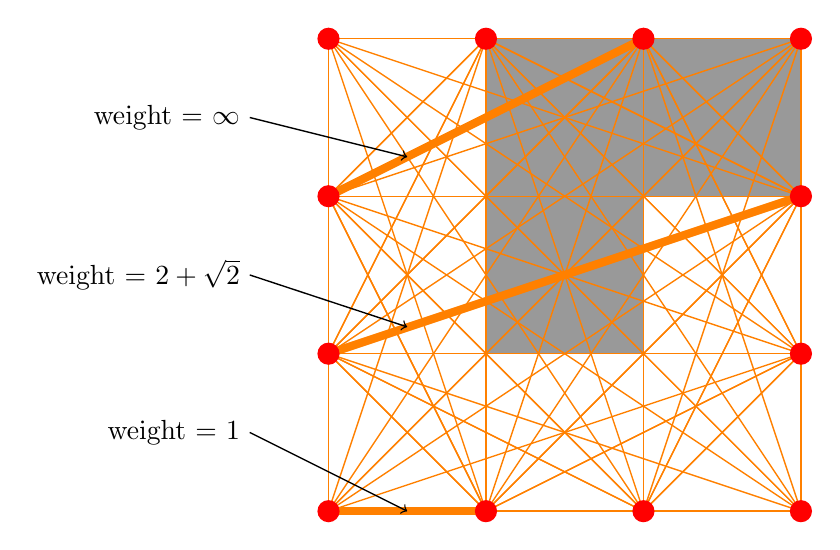
\begin{tikzpicture}[scale=2,line width=0.5pt]
    
      \filldraw[color=black!60,fill=black!40] (1,1) rectangle (2,3); 
      \filldraw[color=black!60,fill=black!40] (1,2) rectangle (3,3); 
  
      \foreach \x in {0,1,2,3} {
        \foreach \y in {0} {
          \foreach \a in {0,1,2,3} {
            \foreach \b in {3} {
              \draw[orange] (\x,\y) -- (\a,\b);
              \draw[orange] (\y,\x) -- (\b,\a);
            }
          }
        }
      }
      
      \foreach \x in {1,2} {
        \foreach \y in {0,3} {
          \foreach \a in {0,3} {
            \foreach \b in {1,2} {
              \draw[orange] (\x,\y) -- (\a,\b);
              \draw[orange] (\y,\x) -- (\b,\a);
            }
          }
        }
      }
      
      \draw[orange, line width = 3pt] (0,0) -- (1,0);
      \draw[orange, line width = 3pt](0,1) -- (3,2);
      \draw[orange, line width = 3pt] (0,2) -- (2,3);
      
      \node[left] at (-0.5,0.5) {weight = $1$};
      \draw[->] (-0.5,0.5) -- (0.5,0);
      \node[left] at (-0.5,1.5) {weight = $2 + \sqrt 2$};
      \draw[->] (-0.5,1.5) -- (0.5,1.17);
      \node[left] at (-0.5,2.5) {weight = $\infty$};
      \draw[->] (-0.5,2.5) -- (0.5,2.25);
      
      \fill[red] (0,0) circle (2pt);
      \fill[red] (0,1) circle (2pt);
      \fill[red] (0,2) circle (2pt);
      \fill[red] (0,3) circle (2pt);
      \fill[red] (3,0) circle (2pt);
      \fill[red] (3,1) circle (2pt);
      \fill[red] (3,2) circle (2pt);
      \fill[red] (3,3) circle (2pt);
      \fill[red] (1,0) circle (2pt);
      \fill[red] (2,0) circle (2pt);
      \fill[red] (1,3) circle (2pt);
      \fill[red] (2,3) circle (2pt);
      
     
    \end{tikzpicture}
    \caption[Anatomy of a block]{A block of size $3^{2}$ laid over the area of map it represents, with certain highlighted edge weights labeled.}
  %\label{fig:fig}
\end{figure}

\noindent
The edge weights for regular blocks are discovered by querying the {\em Local Distance Database (LDDB)}, which is introduced in the next subsection. Since the {\em LDDB} only contains data for regular blocks, the weights of edges in $B_{start}$ and $B_{goal}$ are calculated separately --- this is discussed in the {\bfseries Implementation} chapter of this dissertation.\\

\noindent
Each block $B_{i,j}$ contains nodes that are collocational with nodes from up to six neighbouring blocks. Figure 2.6 shows collocational nodes as two or four partially overlapping red circles. {\em Block A*} maintains the invariant for two collocational nodes $n$ and $n'$ that $n.g = n'.g$ and $n.h = n'.h$ --- the enforcement of this invariant enables shortest path information to flow between adjacent blocks.\\

\noindent
{\bfseries Local Distance Database (LDDB)}\\
\noindent
An $LDDB_{N}$ is a pre-computed database that holds the path length and inflection points of the optimum paths between all pairs of locations $(a,b)$ and $(c,d)$ for all map configurations $M$ of size $N^{2}$, where $a,b,c,d \in \mathbb{Z}$ and $(a,b)$ and $(c,d)$ lie on the boundary of $M$.\\

\noindent
{\bfseries Initialisation}\\
\noindent
For all $n \in B_{start}$, $n.g$ is set to $(n_{start},n).weight$. For all $n \in B_{goal}$, $n.h$ is set to $(n,n_{goal}).weight$. Since there is no guarantee that $n_{start}$ and $n_{goal}$ lie on the boundary of a block, these edge weights cannot be obtained from the $LDDB$, but must be calculated separately. The exceptional case that $B_{start} = B_{goal}$ must also be checked for. Both of these issues are discussed in the {\bfseries Implementation} chapter.\\

\noindent
Having initialised $B_{start}$ and $B_{goal}$, $B_{start}$ is added to $openSet$.\\

\noindent
{\bfseries Iteration}\\
\noindent
The iteration stage of {\em Block A*} proceeds similarly to {\em A*}, though {\em Block A*} expands blocks chosen from $openSet_{blocks}$ whereas {\em A*} expands nodes. However, note that a block can be expanded multiple times, whereas in {\em A*} a node is only expanded once. Therefore, the shortest path may not have been reached when $B_{goal}$ is first expanded, hence the expansion of $B_{goal}$ cannot be used as a termination condition. Therefore a $length$ variable is maintained, which ensures that the algorithm terminates only when it is impossible to find a shorter path.\\

\noindent
{\bfseries Expansion}\\
\noindent
On expansion of $B_{i,j}$, {\em Block A*} attempts to relax every edge $e=(n_{ingress},n_{egress}) \in E_{i,j}$ where $n_{ingress} \in openSet_{i,j}$ and $n_{egress} \in V_{i,j}$. If $e$ is relaxed, all nodes that are collocational with $n_{egress}$ are added to the $openSet_{k,l}$ of their respective block $B_{k,l}$, and $B_{k,l}$ is added to $openSet$ if it is not already a member. \\

\noindent
{\bfseries Termination}\\
\noindent
The {\em h-value} of $B_{goal}$ is the actual shortest path from each node $n \in V_{goal}$, (see {\bfseries Initialisation} subsection) as opposed to a Euclidean estimate that is used for the {\em h-value} in every other block. Therefore, if $B_{goal}.heapValue$ is less than the $heapValue$ of any other blocks in $openSet$ then there are no possible shorter paths to $B_{goal}$, so the algorithm terminates. This condition is ensured by the $length$ variable.\\

\noindent
{\bfseries Traceback}\\
\noindent
When {\em Block A*} terminates, the boundary nodes of the blocks through which $P_{G_{M}}$ passes can be found by recursively following the $parent$ pointers from $n_{goal}$ to $n_{start}$. See figure 2.8 (b). However, to recover the nodes of $P_{G_{M}}$ that do not lie on the boundaries of blocks, a traceback stage is required which involves multiple queries to the $LDDB$. See figure 2.8 (c). Although the details of this are not presented in Yap's paper, an explanation is presented in the {\bfseries Implementation} chapter of this dissertation.\\

\begin{algorithm}
  \SetAlgoLined\DontPrintSemicolon
  \SetKwFunction{bAS}{BlockAStar}\SetKwFunction{expand}{Expand}\SetKwFunction{traceback}{TraceBack}
  \SetKwProg{myDef}{def}{}{}
  \myDef{\bAS{G, $n_{start}$, $n_{goal}$}}{
  \nl $B_{start} \gets init(n_{start})$\;
  \nl $B_{goal} \gets init(n_{goal})$\;
  \nl $length \gets \infty$\;
  \nl $openSet_{blocks}.add(B_{start})$\;
  \nl \While{$(openSet_{blocks} \neq \bot) \land ((openSet_{blocks}.peek()).heapValue < length)$} {
    \nl $B_{curr} \gets openSet_{blocks}.pop()$\;
    \nl $openSet_{curr} \gets B_{curr}.openSet$\;
    \nl \If{$B_{curr} = B_{goal}$} {
      \nl $length \gets \min\limits_{n \in openSet_{curr}} (n.g + euclidean(n,n_{goal}),length)$\;
    }
    \nl $\expand(B_{curr},openSet_{curr})$\;
  }
  \nl \uIf{$length \neq \infty$}{
    \nl $\traceback(n_{goal})$\;
  } \nl \Else {
     \nl \KwRet{$\bot$}\;
  }
}{}

 \setcounter{AlgoLine}{0}
  \myDef{\expand{$B_{curr},openSet_{curr}$}}{
    \nl \While{$openSet_{curr} \neq \bot $}{
      \nl $n_{ingress} \gets openSet_{curr}.pop()$\;
      \nl \ForEach{$n_{egress} \in B_{curr}$}{
        \nl \uIf{$n_{ingress}.g + (n_{ingress},n_{egress}).weight < n_{egress}.g$} {
          \nl $n_{egress}.g \gets n_{ingress}.g + (n_{ingress},n_{egress}).weight$\;
            \nl \ForEach{$n' \in n_{egress}.collocational$}{
              \nl $n' \gets n_{ingress}.g + (n_{ingress},n_{egress}).weight$\;
              \nl $openSet_{n'.coord}.add(n')$\;
              \nl \uIf{$openSet_{blocks}.contains(B_{n'.coord}) = false$} {
                \nl $openSet_{blocks}.add(B_{n'.coord})$\;
              }
            }
        }
      }
    }
  }
 
  \caption{{\sc Block A*}}
\end{algorithm} 


\begin{figure}
    \centering
    \begin{tikzpicture}
    
\node (a) at (0,10) {
    	\begin{tikzpicture}[scale=0.85,line width=0.5pt]
	      	\filldraw[color=black!60,fill=black!40] (0,0) rectangle (2,3); 
		\filldraw[color=black!60,fill=black!40] (1,7) rectangle (8,8); 
		\filldraw[color=black!60,fill=black!40] (7,7) rectangle (8,5); 
		\filldraw[color=black!60,fill=black!40] (2,4) rectangle (5,6);
		\filldraw[color=black!60,fill=black!40] (3,2) rectangle (5,4); 
		\filldraw[color=black!60,fill=black!40] (4,1) rectangle (5,2);  
     	 	\draw[color=black!60] (0,0) grid (9,9);
      		\draw[black] (0,0) -- (0,9);
      		\draw[black] (0,0) -- (9,0);
      		\draw[black] (9,9) -- (0,9);
      		\draw[black] (9,9) -- (9,0);
		\fill[blue] (1,4) circle (3pt);
		\node[below left] at (1,4) {$start$};
		\fill[blue] (8,2) circle (3pt);
		\node[below left] at (8,2) {$goal$};
		
		\node at (4.5,-1) {(a) Original map $M$};
	    \end{tikzpicture}
	    };	   
	   
\node (b) at (10,10) {
    	    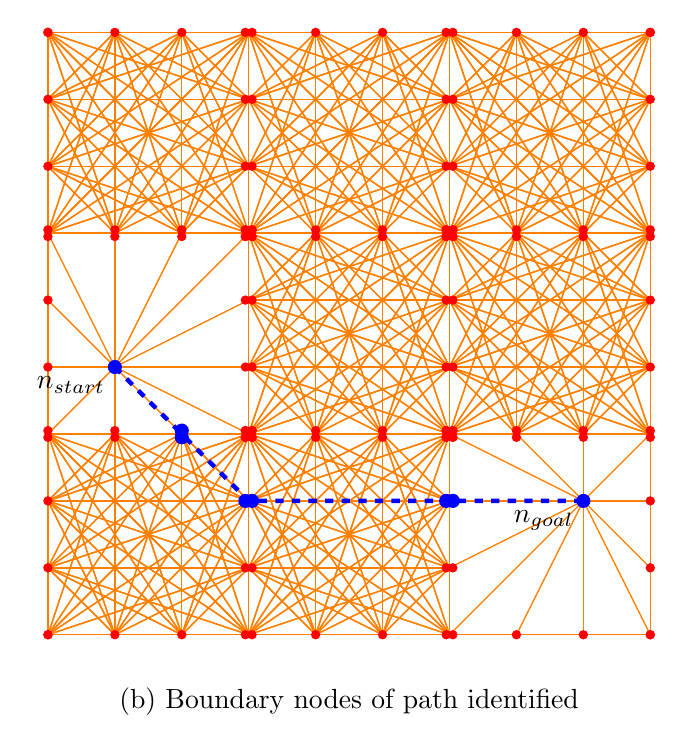
\begin{tikzpicture}[scale=0.85,line width=0.5pt]
  
      \foreach \i in {0,3,6} {
      \foreach \j in {0,3,6} {
      \foreach \x in {0,1,2,3} {
        \foreach \y in {0,3} {
          \foreach \a in {0,1,2,3} {
            \foreach \b in {0,3} {
             \pgfmathparse{int(\x + \i)};
             \let\xn\pgfmathresult;
             \pgfmathparse{int(\a + \i)};
             \let\an\pgfmathresult;
             \pgfmathparse{int(\y + \j)};
             \let\yn\pgfmathresult;
             \pgfmathparse{int(\b + \j)};
             \let\bn\pgfmathresult;
              \draw[orange] (\xn,\yn) -- (\an,\bn);
              \draw[orange] (\yn,\xn) -- (\bn,\an);
            }
          }
        }
      }
      }}
      
      \foreach \i in {0,3,6} {
      \foreach \j in {0,3,6} {
      \foreach \x in {1,2} {
        \foreach \y in {0,3} {
          \foreach \a in {1,2} {
            \foreach \b in {0,3} {
             \pgfmathparse{int(\x+\i)};
             \let\xn\pgfmathresult;
             \pgfmathparse{int(\a+\j)};
             \let\an\pgfmathresult;
             \pgfmathparse{int(\y+\j)};
             \let\yn\pgfmathresult;
             \pgfmathparse{int(\b+\i)};
             \let\bn\pgfmathresult;
              \draw[orange] (\xn,\yn) -- (\bn,\an);
              \draw[orange] (\yn,\xn) -- (\an,\bn);
            }
          }
        }
      }
      }}
      
      \filldraw[color=orange, fill=white] (0,3) rectangle (3,6);
      \filldraw[color=orange, fill=white] (6,0) rectangle (9,3);
      
      \draw[orange] (1,4) -- (0,3);
      \draw[orange] (1,4) -- (0,4);
      \draw[orange] (1,4) -- (0,5);
      \draw[orange] (1,4) -- (0,6);
      \draw[orange] (1,4) -- (3,3);
      \draw[orange] (1,4) -- (3,4);
      \draw[orange] (1,4) -- (3,5);
      \draw[orange] (1,4) -- (3,6);
      \draw[orange] (1,4) -- (1,3);
      \draw[orange] (1,4) -- (2,3);
      \draw[orange] (1,4) -- (1,6);
      \draw[orange] (1,4) -- (2,6);

      \draw[orange] (8,2) -- (6,0);
      \draw[orange] (8,2) -- (6,1);
      \draw[orange] (8,2) -- (6,2);
      \draw[orange] (8,2) -- (6,3);
      \draw[orange] (8,2) -- (9,0);
      \draw[orange] (8,2) -- (9,1);
      \draw[orange] (8,2) -- (9,2);
      \draw[orange] (8,2) -- (9,3);
      \draw[orange] (8,2) -- (7,0);
      \draw[orange] (8,2) -- (8,0);
      \draw[orange] (8,2) -- (7,3);
      \draw[orange] (8,2) -- (8,3);     
      
      \fill[red] (1,4) circle (2pt);
      \node[below left] at (1,4) {$n_{start}$};
      \fill[red] (8,2) circle (2pt);
      \node[below left] at (8,2) {$n_{goal}$};
      
      \foreach \x in {0,1,2,2.95,3.05,4,5,5.95,6.05,7,8,9} {
        \foreach \y in {0,9} {
              \fill[red] (\x,\y) circle (2pt);
              \fill[red] (\y,\x) circle (2pt);
        }
      }
      
      \foreach \x in {1,2,4,5,7,8} {
        \foreach \y in {3,6} {
          \pgfmathparse{(\y + 0.05)};
           \let\ya\pgfmathresult;
            \pgfmathparse{(\y - 0.05)};
           \let\yb\pgfmathresult;
              \fill[red] (\x,\ya) circle (2pt);
              \fill[red] (\x,\yb) circle (2pt);
              \fill[red] (\ya,\x) circle (2pt);
              \fill[red] (\yb,\x) circle (2pt);
        }
      }
      
       \foreach \x in {3,6} {
        \foreach \y in {3,6} {
          \pgfmathparse{(\x + 0.05)};
           \let\xa\pgfmathresult;
            \pgfmathparse{(\x - 0.05)};
           \let\xb\pgfmathresult;
           \pgfmathparse{(\y + 0.05)};
           \let\ya\pgfmathresult;
              \fill[red] (\xa,\ya) circle (2pt);
              \fill[red] (\xb,\ya) circle (2pt);
              \fill[red] (\ya,\xa) circle (2pt);
              \fill[red] (\ya,\xb) circle (2pt);
        }
      }
      
             \foreach \x in {3,6} {
        \foreach \y in {3,6} {
          \pgfmathparse{(\x + 0.05)};
           \let\xa\pgfmathresult;
            \pgfmathparse{(\x - 0.05)};
           \let\xb\pgfmathresult;
           \pgfmathparse{(\y - 0.05)};
           \let\ya\pgfmathresult;
              \fill[red] (\xa,\ya) circle (2pt);
              \fill[red] (\xb,\ya) circle (2pt);
              \fill[red] (\ya,\xa) circle (2pt);
              \fill[red] (\ya,\xb) circle (2pt);
        }
      }
      
      \fill[blue] (1,4) circle (3pt);
      \fill[blue] (2,3.05) circle (3pt);
      \fill[blue] (2,2.95) circle (3pt);
      \fill[blue] (2.95,2) circle (3pt);
      \fill[blue] (3.05,2) circle (3pt);
      \fill[blue] (5.95,2) circle (3pt);
      \fill[blue] (6.05,2) circle (3pt);
      \fill[blue] (8,2) circle (3pt);
      \draw[blue,ultra thick,dashed] (1,4) -- (2,3) -- (3,2) -- (6,2) -- (8,2);
      
      \node at (4.5,-1) {(b) Boundary nodes of path identified};
     
    \end{tikzpicture}
	    };
	    
\node (c) at (0,0) {
    	    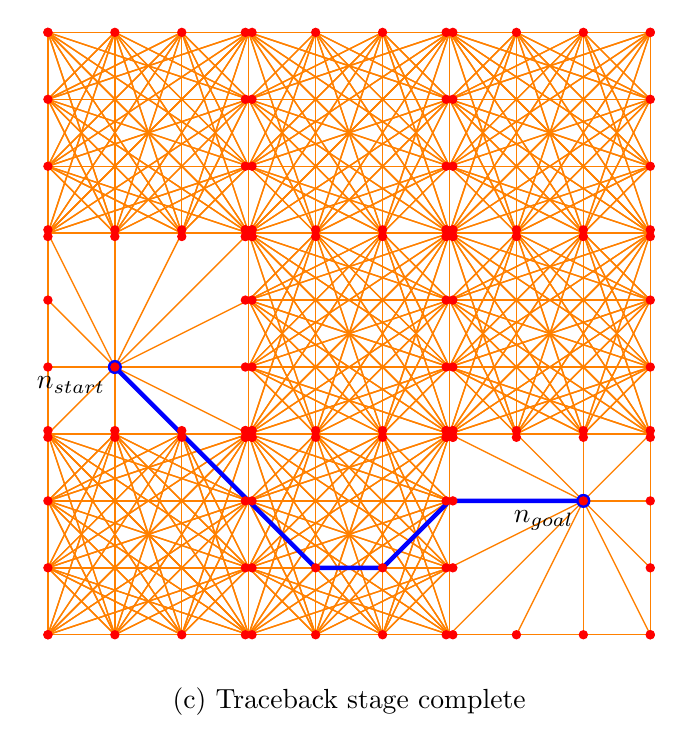
\begin{tikzpicture}[scale=0.85,line width=0.5pt]
  
      \foreach \i in {0,3,6} {
      \foreach \j in {0,3,6} {
      \foreach \x in {0,1,2,3} {
        \foreach \y in {0,3} {
          \foreach \a in {0,1,2,3} {
            \foreach \b in {0,3} {
             \pgfmathparse{int(\x + \i)};
             \let\xn\pgfmathresult;
             \pgfmathparse{int(\a + \i)};
             \let\an\pgfmathresult;
             \pgfmathparse{int(\y + \j)};
             \let\yn\pgfmathresult;
             \pgfmathparse{int(\b + \j)};
             \let\bn\pgfmathresult;
              \draw[orange] (\xn,\yn) -- (\an,\bn);
              \draw[orange] (\yn,\xn) -- (\bn,\an);
            }
          }
        }
      }
      }}
      
      \foreach \i in {0,3,6} {
      \foreach \j in {0,3,6} {
      \foreach \x in {1,2} {
        \foreach \y in {0,3} {
          \foreach \a in {1,2} {
            \foreach \b in {0,3} {
             \pgfmathparse{int(\x+\i)};
             \let\xn\pgfmathresult;
             \pgfmathparse{int(\a+\j)};
             \let\an\pgfmathresult;
             \pgfmathparse{int(\y+\j)};
             \let\yn\pgfmathresult;
             \pgfmathparse{int(\b+\i)};
             \let\bn\pgfmathresult;
              \draw[orange] (\xn,\yn) -- (\bn,\an);
              \draw[orange] (\yn,\xn) -- (\an,\bn);
            }
          }
        }
      }
      }}
      
      \filldraw[color=orange, fill=white] (0,3) rectangle (3,6);
      \filldraw[color=orange, fill=white] (6,0) rectangle (9,3);
      
      \draw[orange] (1,4) -- (0,3);
      \draw[orange] (1,4) -- (0,4);
      \draw[orange] (1,4) -- (0,5);
      \draw[orange] (1,4) -- (0,6);
      \draw[orange] (1,4) -- (3,3);
      \draw[orange] (1,4) -- (3,4);
      \draw[orange] (1,4) -- (3,5);
      \draw[orange] (1,4) -- (3,6);
      \draw[orange] (1,4) -- (1,3);
      \draw[orange] (1,4) -- (2,3);
      \draw[orange] (1,4) -- (1,6);
      \draw[orange] (1,4) -- (2,6);

      \draw[orange] (8,2) -- (6,0);
      \draw[orange] (8,2) -- (6,1);
      \draw[orange] (8,2) -- (6,2);
      \draw[orange] (8,2) -- (6,3);
      \draw[orange] (8,2) -- (9,0);
      \draw[orange] (8,2) -- (9,1);
      \draw[orange] (8,2) -- (9,2);
      \draw[orange] (8,2) -- (9,3);
      \draw[orange] (8,2) -- (7,0);
      \draw[orange] (8,2) -- (8,0);
      \draw[orange] (8,2) -- (7,3);
      \draw[orange] (8,2) -- (8,3);   
      
      \draw[blue,ultra thick] (1,4) -- (2,3) -- (3,2) -- (4,1) -- (5,1) -- (6,2) -- (8,2);
      \fill[blue] (1,4) circle (3pt);
      \fill[blue] (8,2) circle (3pt);
      \fill[red] (4,1) circle (2pt);
      \fill[red] (5,1) circle (2pt);
      
      \fill[red] (1,4) circle (2pt);
      \node[below left] at (1,4) {$n_{start}$};
      \fill[red] (8,2) circle (2pt);
      \node[below left] at (8,2) {$n_{goal}$};
      
      \foreach \x in {0,1,2,2.95,3.05,4,5,5.95,6.05,7,8,9} {
        \foreach \y in {0,9} {
              \fill[red] (\x,\y) circle (2pt);
              \fill[red] (\y,\x) circle (2pt);
        }
      }
      
      \foreach \x in {1,2,4,5,7,8} {
        \foreach \y in {3,6} {
          \pgfmathparse{(\y + 0.05)};
           \let\ya\pgfmathresult;
            \pgfmathparse{(\y - 0.05)};
           \let\yb\pgfmathresult;
              \fill[red] (\x,\ya) circle (2pt);
              \fill[red] (\x,\yb) circle (2pt);
              \fill[red] (\ya,\x) circle (2pt);
              \fill[red] (\yb,\x) circle (2pt);
        }
      }
      
       \foreach \x in {3,6} {
        \foreach \y in {3,6} {
          \pgfmathparse{(\x + 0.05)};
           \let\xa\pgfmathresult;
            \pgfmathparse{(\x - 0.05)};
           \let\xb\pgfmathresult;
           \pgfmathparse{(\y + 0.05)};
           \let\ya\pgfmathresult;
              \fill[red] (\xa,\ya) circle (2pt);
              \fill[red] (\xb,\ya) circle (2pt);
              \fill[red] (\ya,\xa) circle (2pt);
              \fill[red] (\ya,\xb) circle (2pt);
        }
      }
      
             \foreach \x in {3,6} {
        \foreach \y in {3,6} {
          \pgfmathparse{(\x + 0.05)};
           \let\xa\pgfmathresult;
            \pgfmathparse{(\x - 0.05)};
           \let\xb\pgfmathresult;
           \pgfmathparse{(\y - 0.05)};
           \let\ya\pgfmathresult;
              \fill[red] (\xa,\ya) circle (2pt);
              \fill[red] (\xb,\ya) circle (2pt);
              \fill[red] (\ya,\xa) circle (2pt);
              \fill[red] (\ya,\xb) circle (2pt);
        }
      }
      
      \node at (4.5,-1) {(c) Traceback stage complete};
      
     
    \end{tikzpicture}
	    };
	    
\node (d) at (10,0) {
    	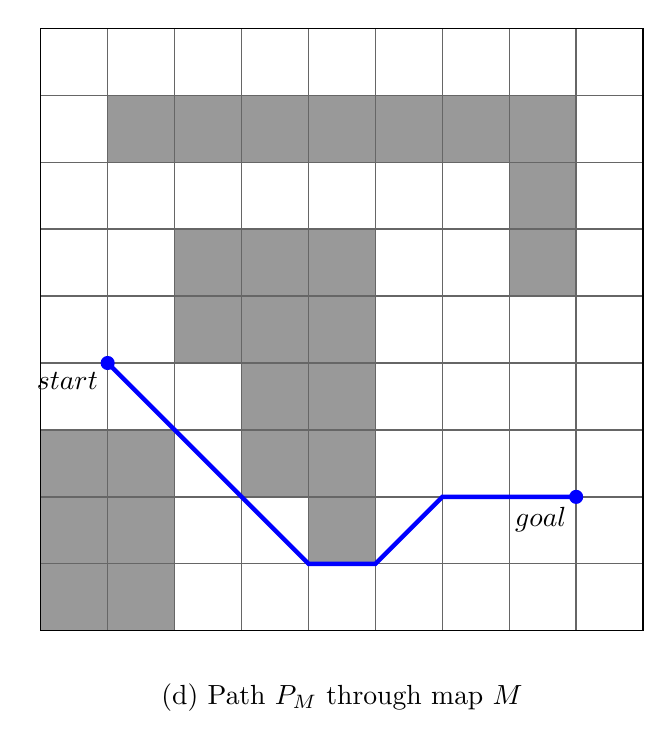
\begin{tikzpicture}[scale=0.85,line width=0.5pt]
	      	\filldraw[color=black!60,fill=black!40] (0,0) rectangle (2,3); 
		\filldraw[color=black!60,fill=black!40] (1,7) rectangle (8,8); 
		\filldraw[color=black!60,fill=black!40] (7,7) rectangle (8,5); 
		\filldraw[color=black!60,fill=black!40] (2,4) rectangle (5,6);
		\filldraw[color=black!60,fill=black!40] (3,2) rectangle (5,4); 
		\filldraw[color=black!60,fill=black!40] (4,1) rectangle (5,2);  
     	 	\draw[color=black!60] (0,0) grid (9,9);
      		\draw[black] (0,0) -- (0,9);
      		\draw[black] (0,0) -- (9,0);
      		\draw[black] (9,9) -- (0,9);
      		\draw[black] (9,9) -- (9,0);
		\node[below left] at (1,4) {$start$};
		\node[below left] at (8,2) {$goal$};
		\fill[blue] (1,4) circle (3pt);
      		\fill[blue] (8,2) circle (3pt);
      		\draw[blue,ultra thick] (1,4) -- (2,3) -- (3,2) -- (4,1) -- (5,1) -- (6,2) -- (8,2);
		
		\node at (4.5,-1) {(d) Path $P_{M}$ through map $M$};
	    \end{tikzpicture}
	    };	

    \end{tikzpicture}
    \caption[Solution of {\em Block A*}]{Solution of {\em Block A*}}
  %\label{fig:fig}
\end{figure}


\clearpage
\section {Requirements analysis}

As specified in the {\bfseries Work to be done} section of the {\bfseries Proposal} (see {\bfseries Appendix E}), this project is logically composed of four parts. This section outlines the functional and non-functional requirements for each part, and their relative priorities using the MoSCoW system. \\
\centerline {{\bf M} - Must; {\bf S} - Should; {\bf C} - Could; {\bf W} - Won't}

\subsection{Testing simulator}

\begin{center}
    \begin{tabular}{ l | p{10cm} | l}
    ID & Functional requirement & Priority  \\ \hline
    1 & The system shall load one of a collection of maps from the generator & M \\ \hline
    2 & The system shall load one of a collection of maps from a saved file & S \\ \hline
    3 & The system shall create a grid-graph from a given map & M \\ \hline
    4 & The system shall create a visibility graph from a given map & C \\ \hline
    5 & The system shall run one of a collection of any-angle path-finding algorithms on a graph and collect data such as the path-length and the length of computation & M \\ \hline
    6 & The system shall display a visual representation of the current map and the paths found by any algorithms that have been run on it & M \\ \hline
    7 & The system shall display the numeric statistics for each path for the current map & M \\ \hline
     \hline 
    ID & Non-functional requirement & Priority  \\ \hline
    1 & The system shall be designed in a modular way to allow easy extension for new algorithms & S \\
    \end{tabular}
\end{center}

\subsection{Map generation}

\begin{center}
    \begin{tabular}{ l | p{10cm} | l }
    ID & Functional requirement & Priority  \\ \hline
    1 & The system shall generate pseudo-random maps of a given resolution, coverage percentage and clustering & M \\ \hline
    2 & The system shall allow maps to be saved so that multiple tests can be run on the same map suite & M \\ \hline
     3 & The system shall allow maps to be created with an interactive map editor & C\\ \hline
          \hline 
    ID & Non-functional requirement & Priority  \\ \hline
    1 & The system shall generate maps of the highest resolution in under 2 seconds & S \\
    \end{tabular}
\end{center}
	
\subsection{Algorithm implementation}

\begin{center}
    \begin{tabular}{ l | p{10cm} | l}
    ID & Functional requirement & Priority  \\ \hline
    1 & The system shall correctly implement each of the chosen algorithms. If a path exists, the path and numerical statistics will be returned. If no path exists, this will be returned   & M \\ \hline
    2 & The system shall allow arbitrary start and end coordinates for any map & S \\ \hline
     \hline 
    ID & Non-functional requirement & Priority  \\ \hline
    1 & The system shall be designed in a modular way to allow easy extension for new algorithms & S \\
    \end{tabular}
\end{center}

\subsection{Data gathering}

\begin{center}
    \begin{tabular}{ l | p{10cm} | l}
    ID & Functional requirement & Priority  \\ \hline
    1 & The system shall write statistics for an arbitrary set of specified algorithms on an arbitrary set of specified maps and write the results to a CSV file & M \\ \hline
     \hline 
    ID & Non-functional requirement & Priority  \\ \hline
    1 & The system shall be designed with a clear API that enables quick and easy data gathering. & M \\
    \end{tabular}
\end{center}

\noindent
\missingfigure{UML diagrams - use case and sequence diagram etc}

\section {Testing}

A thorough testing strategy was devised to reduce the chances of bugs being introduced into the code. Separate strategies were required for different modules of the system:

\begin{description}
\item[Simulator]\hfil \\
{\em Core structural classes} --- basic functionality to be unit tested;\\
{\em Line of sight algorithm} --- to be unit tested thoroughly, as its correctness will be assumed during testing of pathfinding algorithm implementations;\\
{\em Pathfinding algorithms} --- correctness of all paths returned by to be optionally verified.
\end{description}
\begin{description}
\item[User interface]\hfil \\
{\em Use case scenarios} --- to be manually tested by human user.
\end{description}
\begin{description}
\item[Data extraction scripts]\hfil \\
{\em Exported CSVs} --- contents of CSV files to be unit tested.
\end{description}

\section {Design model}

\noindent
Once the preparation phase of the project was completed, the plan for the implementation phase was refined from that presented in the Project Proposal (see Appendix ?). An incremental model of implementation was adopted, with new modules being developed and tested separately before being integrated into the work program. The milestones of the project were:
\begin{description}
\item[Milestone 1]\hfil \\
Maps of arbitrary size, coverage and clustering can be created and printed to system output.
\item[Milestone 2]\hfil \\
Arbitrary maps can be converted to graphs, and {\em Dijkstra} and {\em A*} can be run on these maps. A visual representation of the path can be printed to system output.
\item[Milestone 3]\hfil \\
Basic UI is built, including all functionality from {\bfseries Milestone 2}. Basic path statistics are displayed.
\item[Milestone 4]\hfil \\
Map saving, map loading and map creation functionality are present. This will facilitate debugging edge cases for more complex algorithms.
\item[Milestone 5]\hfil \\
{\em A* with post-smoothing}, {\em Theta*} and {\em Lazy Theta*} are implemented.
\item[Milestone 6]\hfil \\
{\em Block A*} is implemented.
\item[Milestone 7]\hfil \\
Data extraction scripts are implemented.
\end{description}

\section {Languages and tools}

This section justifies the languages, libraries and tools that were chosen for this project.

\begin{description}
  \item[Programming language] \hfill \\
  {\em Java} --- provides abstraction and class hierarchy to enable development of modular, extensible code.
  \item[Libraries] \hfill \\
  {\em Swing} --- for graphical user interface design;\\ 
  {\em CSVWriter} --- for data export;\\
  {\em JUnit} --- for unit testing.
  \item[Integrated development environment] \hfill \\
  {\em Eclipse} --- allows rapid development through integrated testing, refactoring and version control tools.
  \item[Statistical analysis and visualisation] \hfill \\
  {\em R} --- open-source statistical package; chosen due to its flexibility and extensibility.
  \item[Document preparation] \hfill \\
  {\LaTeX} --- allows precise, integrated control over all aspects of document layout and style;\\
  {\em Tikz} --- drawing package for \LaTeX\ that enables programmable diagram creation;\\
  {\em algorithm2e} --- pseudo-code package for \LaTeX\ that enables integration with the parent document.
  \item[Backup] \hfill \\
  {\em DropBox} and {\em Google Drive} --- maintain multiple shadow copies of my work in the cloud.
  \item[Version Control]\hfill \\
  {\em GitHub} --- facilitated exploring different implementation strategies by forking my core code repository.
  
\end{description}

%\cleardoublepage
\chapter{Implementation}

This chapter provides an overview of the implementation of the project and explores some of the more interesting parts in further detail.\\

\noindent
Figure 3.1 provides an simplified view of the flow of the user interface and engine of the program. This simplified view only communicates the core interactions between the user interface and the engine, and is included to serve as a useful framework with which to describe the implementation of the program. The more complex interactions between the user interface and the engine were derived from the Use Cases, some of which are given in the {\bfseries ?} section of the {\bfseries Preparation} chapter, and are explained in greater detail in some of the sections of this chapter.\\

\noindent
The basic control flow upon which figure 3.1 is based is explained below:
\begin{itemize}
\item {\bfseries Map \& algorithm selection} --- the user selects a map using one of the three methods below, selects a start and goal point and selects an pathfinding algorithm.
  \begin{itemize}
  \item {\bfseries MapGenerator} --- allows the program to automatically generate a map according to user-selected parameters;
  \item {\bfseries MapCreator} --- creates the map using a `paint brush' style editor;
  \item {\bfseries MapLoader} --- loads a map that has been previously saved;
  \end{itemize}
\item {\bfseries GraphGenerator} --- the system creates a graph representation of the map;
\item {\bfseries Pathfinding algorithm} --- the system runs the selected pathfinding algorithm on the graph;
\item {\bfseries Visualizer} --- the system displays the path, and statistics about the path, in the visualiser;
\item {\bfseries Data export} --- the statistics about the path may be exported in CSV format.
\end{itemize}

\begin{figure}[h]
  \centering
  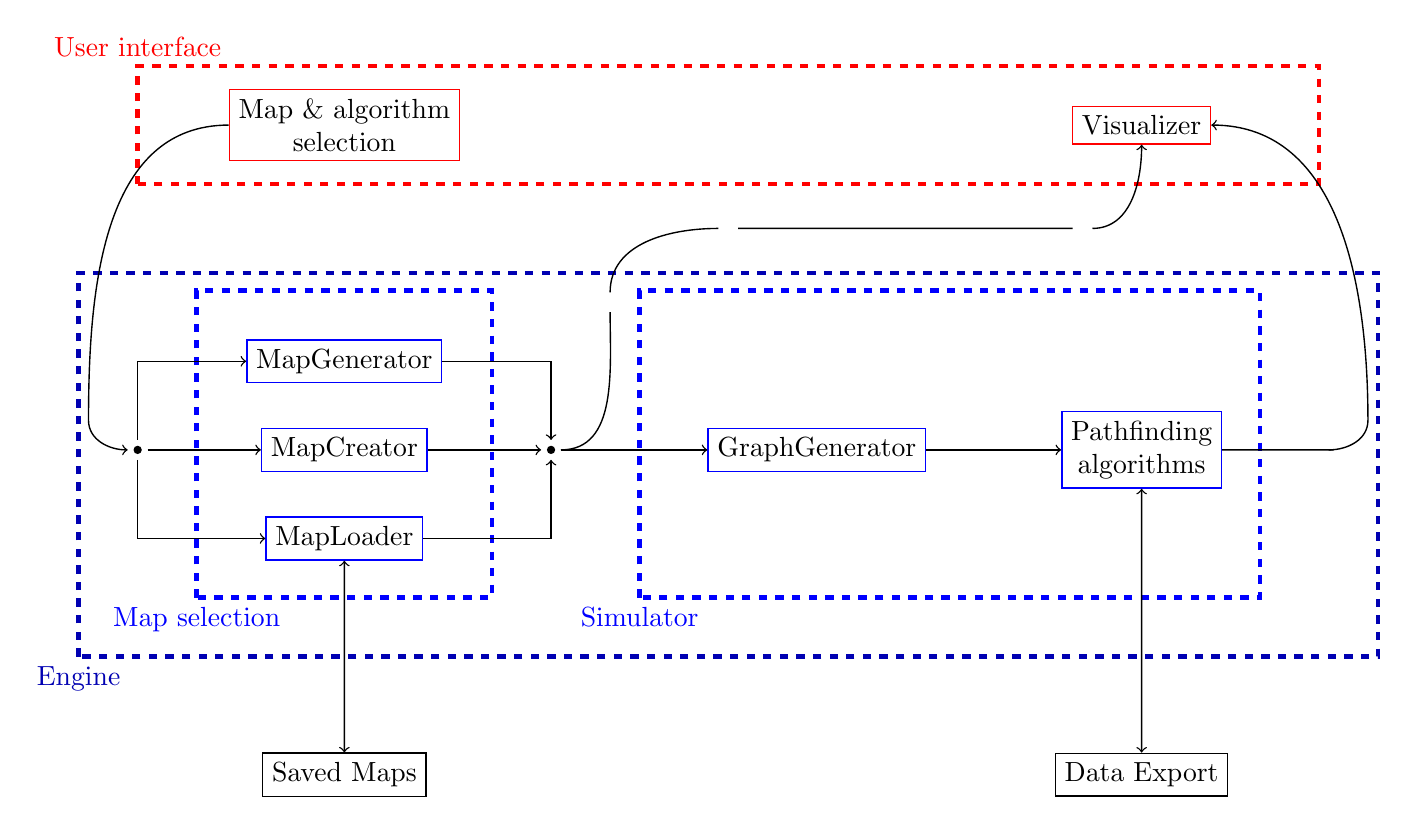
\begin{tikzpicture}[scale=0.75,line width=0.5pt]
  \filldraw[color=red,fill=white,dashed, ultra thick] (0,5) rectangle (20,7); 
  \node[above, red] at (0,7) {User interface};
  \filldraw[color=blue!70!black,fill=white,dashed, ultra thick] (-1,-3) rectangle (21,3.5); 
  \node[below, blue!70!black] at (-1,-3) {Engine};
  \filldraw[color=blue,fill=white,dashed, ultra thick] (1,-2) rectangle (6,3.2); 
  \node[below, blue] at (1,-2) {Map selection};
  \filldraw[color=blue,fill=white,dashed, ultra thick] (8.5,-2) rectangle (19,3.2); 
  \node[below, blue] at (8.5,-2) {Simulator};
  
\node[draw=red,shape=rectangle,align=center] at (3.5,6) (MapAlgSelection) {Map \& algorithm \\selection};
\node at (-1,1) (LeftCurveNode) {};
\fill (0,0.5) circle (2pt);
\node at (0,0.5) (LeftCurveEnd) {};
\node[draw=blue,shape=rectangle,align=center] at (3.5,2) (MapGenerator) {MapGenerator};
\node[draw=blue,shape=rectangle,align=center] at (3.5,0.5) (MapCreator) {MapCreator};
\node[draw=blue,shape=rectangle,align=center] at (3.5,-1) (MapLoader) {MapLoader};
\draw[->] (LeftCurveEnd) |- (MapGenerator);
\draw[->] (LeftCurveEnd) to (MapCreator);
\draw[->] (LeftCurveEnd) |- (MapLoader);
\node at (7,0.5) (InternalNode) {};
\fill (7,0.5) circle (2pt);
\draw[->] (MapGenerator) -| (InternalNode);
\draw[->] (MapCreator) to (InternalNode);
\draw[->] (MapLoader) -| (InternalNode);
\node[draw=blue,shape=rectangle,align=center] at (11.5,0.5) (GraphGenerator) {GraphGenerator};
\draw[->] (InternalNode) to (GraphGenerator);
\node[draw=blue,shape=rectangle,align=center] at (17,0.5) (PathfindingAlgorithms) {Pathfinding \\algorithms};
\draw[->] (GraphGenerator) to (PathfindingAlgorithms);
\node at (20,0.5) (1) {};
\node at (21,1) (RightCurveNode) {};
\draw (PathfindingAlgorithms) to (20.25,0.5);
\node[draw=red,shape=rectangle,align=center] at (17,6) (Visualizer) {Visualizer};
\node at (8,3) (2) {};
\node at (10,4.25) (3) {};
\node at (16,4.25) (4) {};
\draw[->] (InternalNode.east) to[out=0,in=-90] (2) to[out=90,in=180] (3) to[out=0,in=180] (4) to[out=0, in=-90] (Visualizer.south);
\node[draw=black,shape=rectangle,align=center] at (3.5,-5) (SavedMaps) {Saved Maps};
\node[draw=black,shape=rectangle,align=center] at (17,-5) (DataExport) {Data Export};

\draw[->] (MapAlgSelection.west) to[out=180,in=90] (LeftCurveNode.east) to[out=-90,in=180] (LeftCurveEnd.west);
\draw[->] (1.east) to[out=0,in=-90] (RightCurveNode.west) to[out=90,in=0] (Visualizer.east);
\draw[<->] (MapLoader) to (SavedMaps);
\draw[<->] (PathfindingAlgorithms) to (DataExport);


  \end{tikzpicture}
  \caption{Flow of the user interface and engine} 
  \label{fig:lineofsight}
\end{figure}

\section{Map selection}

This section introduces how maps are implemented, and the three methods of selecting a map --- map generation, map creation, and loading a previously saved map.\\

\subsection{Maps}
A map is implemented with a {\tt Map} object, which is a square array of {\tt Cell} objects. Each {\tt Cell} object has a boolean instance variable that records whether or not that cell is blocked.

\subsection{Map generation}
The system provides a module to automatically generate maps according to a given set of parameters, which define the size $N^{2}$ of the map, the percentage $C$ of the cells of the map that are blocked, and a clustering score $D$ which defines how likely the blocked cells are to be found in clusters as opposed to spaced evenly throughout the map. This facility is required so that large volumes of maps can be created to allow for rigorous statistical analysis of the algorithms over maps with certain known properties. A bespoke algorithm was devised for this project to pseudo-randomly create such maps, which is now explained.\\

\missingfigure{Screenshots of maps with different clustering scores}

\noindent
{\bfseries Overview}\\
\noindent
Starting with a blank map (i.e. a map where every cell is free), each iteration of the algorithm chooses one unblocked cell of the map to be blocked, until $C\%$ of the cells have been blocked --- i.e. until $C/N^{2}$ iterations have completed. To record which cells have been blocked on previous iterations and to decide which cell to block on the next iteration, the algorithm maintains a square matrix $m$ of size $N^{2}$, where at any point in the algorithm the value of an element $m_{x,y}$ represents the `potential' of cell $(x,y)$ --- where the potential of an element $m_{x,y}$ represents the relative probability that $(x,y)$ will be chosen to be blocked on the next iteration, or to be more precise: 
\begin{equation}
P((x,y) \mbox{ will be chosen to be blocked on the next iteration}) = m_{x,y}/\sum\limits_{i,j} m_{i,j}
\end{equation}
\noindent
Initially, the potential of every cell is 1, to represent that there is an equal chance of $1/N^{2}$ of any cell being chosen to be blocked in the first iteration of the algorithm.\\

\noindent
If a cell $(x,y)$ is chosen to be blocked, $m_{x,y}$ is set to $0$ to ensure that it cannot be chosen again, and the potentials of the eight cells that surround $(x,y)$ are increased by a value which depends on the clustering score $D$, to ensure that if $D > 0$ then subsequent iterations are more likely to block cells that are spatially close to cells that were blocked on previous iterations, and hence create clusters of blocked cells. The amount by which the potentials of the cells surrounding $(x,y)$ are increased when $(x,y)$ is blocked models a crude approximation of a potential field, or gravity well, around $(x,y)$. See figure 3.2.\todo{insert gravity well figure}\\

\noindent
{\bfseries Implementation}\\
\noindent
A single iteration of the algorithm, which is given in the {\bfseries repeat \ldots until} block in the pseudo-code in {\bfseries Algorithm 7}, can now be summarised: a random number $r$ between $0$ and $\sum\limits_{i,j} m_{i,j}$ is selected, and $m$ is traversed row-by-row until the sum of the potentials of the elements that has been traversed is at least $r$, at which point the traversal stops --- the cell that has been reached is the cell that has been chosen to be blocked. In other words, $(x,y)$ is chosen to be blocked if:
\begin{equation}
(\sum\limits_{((0 \leq i < x) \land (0 \leq j \leq N-1)) \land ((i = x) \land (0 \leq j < y))}m_{i,j} < r) \land (\sum\limits_{((i = x) \land (y < j \leq N-1)) \land ((x < i \leq N-1) \land (0 \leq j \leq N-1))}m_{i,j} < 1-r)
\end{equation}
\noindent
The above is just an implementation of {\em equation 3.1}. Now that $(x,y)$ has been chosen as the cell to be blocked, the potentials of $(x,y)$ and the surrounding eight cells are modified according to the gravity well model (i.e. $m_{x,y}$ is set to $0$, the horizontal neighbours $m_{x-1,y}$, $m_{x+1,y}$ and the vertical neighbours $m_{x,y-1}$ and $m_{x,y+1}$ are increased by $2D$ and the diagonal neighbours $m_{x-1,y-1}$, $m_{x+1,y-1}$, $m_{x+1,y+1}$ and $m_{x-1,y+1}$ are increased by $D$), and the next iteration commences.\\

\noindent
After $C/N^{2}$ iteration, $C\%$ of the cells of the map are blocked, and the algorithm terminates.

\begin{algorithm}
  \SetAlgoLined\DontPrintSemicolon
  \SetKwFunction{genMap}{GenerateMap} \SetKwFunction{setBlocked}{SetAsBlocked}
  \SetKwProg{myDef}{def}{}{}
  \myDef{\genMap{$m, C, D$}}{
    \nl \Repeat{$(C / N^{2}) times$} {
      \nl $r \gets random(0,\sum\limits_{i,j} m_{i,j})$\;
      \nl $i,j \gets 0$\;
      \nl \While{$r\geq 0$} {
        \nl $r \gets r - m_{i,j}$\;
        \nl \uIf{$i < R-1$} {
          \nl $i \gets i+1$\;
        } \nl \Else {
          \nl $i \gets 0$\;
          \nl $j \gets j+1$\;
        }
     }
     \nl \setBlocked{$i,j$};     
  }
  }
  \myDef{\setBlocked{$m_{i,j}$}} {
    \nl $m_{i,j} \gets 0$\;
    \nl \ForEach {$m_{k,l}$ in $horizontalOrVerticalNeighbour(m_{i,j})$} {
      \nl \uIf{$m_{k,l} \neq 0$} {
        \nl $m_{k,l} \gets m_{k,l} + D$\;
      }
  }
  \nl \ForEach {$ m_{k,l}$ in  $diagonalNeighbour(m_{i,j})$} {
      \nl \uIf{$m_{k,l} \neq 0$} {
        $m_{k,l} \gets a_{k,l} + 2\times D$\;
      }
  }
}
\caption{{\sc GenerateMap}}
 \end{algorithm} 
 
 \begin{figure}[h]
\begin{subfigure}{.3\textwidth}
    \centering
    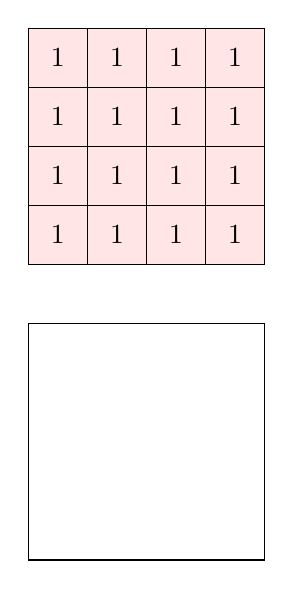
\begin{tikzpicture}[scale=0.75,line width=0.5pt]

     \filldraw[color=red!10] (0,0) rectangle (4,4); 
     \draw (0,0) grid (4,4);
    
     \foreach \x in {0,1,2,3} {
        \foreach \y in {0,1,2,3} {
          \pgfmathparse{(\x + 0.5)};
          \let\xa\pgfmathresult;
          \pgfmathparse{\y + 0.5};
          \let\ya\pgfmathresult;
          \node at (\xa,\ya) {1};
        }
      }
      
      \draw[black] (0,-5) -- (4,-5);
      \draw[black] (0,-5) -- (0,-1);
      \draw[black] (4,-1) -- (4,-5);
      \draw[black] (4,-1) -- (0,-1);
           
    \end{tikzpicture}
    \caption{Initialisation}
    %\label{fig:sfig1}
  \end{subfigure}
  \begin{subfigure}{.3\textwidth}
    \centering
    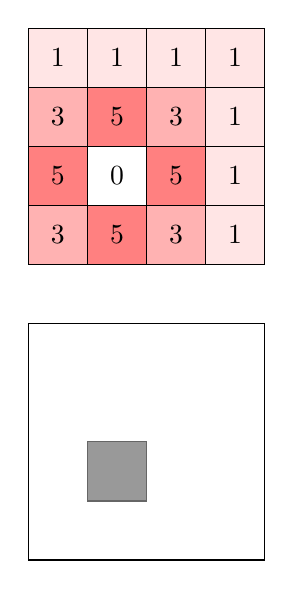
\begin{tikzpicture}[scale=0.75,line width=0.5pt]
    
    \filldraw[color=red!30] (0,0) rectangle (1,1);        
    \node at (0.5,0.5) {3};
    \filldraw[color=red!50] (1,0) rectangle (2,1); 
    \node at (1.5,0.5) {5};
    \filldraw[color=red!30] (2,0) rectangle (3,1); 
    \node at (2.5,0.5) {3};
    \filldraw[color=red!10] (3,0) rectangle (4,1); 
    \node at (3.5,0.5) {1};
    \filldraw[color=red!50] (0,1) rectangle (1,2); 
    \node at (0.5,1.5) {5};
    \filldraw[color=white] (1,1) rectangle (2,2); 
    \node at (1.5,1.5) {0};
    \filldraw[color=red!50] (2,1) rectangle (3,2); 
    \node at (2.5,1.5) {5};
    \filldraw[color=red!10] (3,1) rectangle (4,2); 
    \node at (3.5,1.5) {1};
    \filldraw[color=red!30] (0,2) rectangle (1,3); 
    \node at (0.5,2.5) {3};
    \filldraw[color=red!50] (1,2) rectangle (2,3); 
    \node at (1.5,2.5) {5};
    \filldraw[color=red!30] (2,2) rectangle (3,3); 
    \node at (2.5,2.5) {3};
    \filldraw[color=red!10] (3,2) rectangle (4,3); 
    \node at (3.5,2.5) {1};
    \filldraw[color=red!10] (0,3) rectangle (1,4); 
    \node at (0.5,3.5) {1};
    \filldraw[color=red!10] (1,3) rectangle (2,4); 
    \node at (1.5,3.5) {1};
    \filldraw[color=red!10] (2,3) rectangle (3,4); 
    \node at (2.5,3.5) {1};
    \filldraw[color=red!10] (3,3) rectangle (4,4); 
    \node at (3.5,3.5) {1};

    \draw (0,0) grid (4,4);
    
     \filldraw[color=black!60,fill=black!40] (1,-4) rectangle (2,-3); 
      
      \draw[black] (0,-5) -- (4,-5);
      \draw[black] (0,-5) -- (0,-1);
      \draw[black] (4,-1) -- (4,-5);
      \draw[black] (4,-1) -- (0,-1);
      
    \end{tikzpicture}
    \caption{Iteration 1: r = 5.87}
    %\label{fig:sfig1}
  \end{subfigure}
  %
  \begin{subfigure}{.3\textwidth}
    \centering
    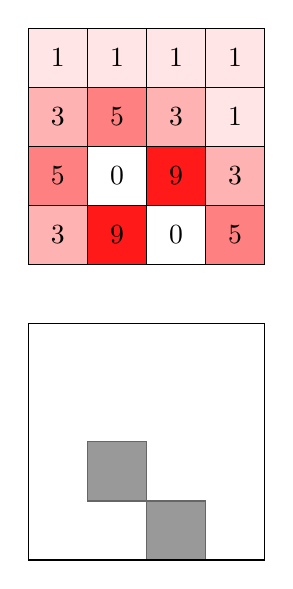
\begin{tikzpicture}[scale=0.75,line width=0.5pt]
    
    \filldraw[color=red!30] (0,0) rectangle (1,1);        
    \node at (0.5,0.5) {3};
    \filldraw[color=red!90] (1,0) rectangle (2,1); 
    \node at (1.5,0.5) {9};
    \filldraw[color=white] (2,0) rectangle (3,1); 
    \node at (2.5,0.5) {0};
    \filldraw[color=red!50] (3,0) rectangle (4,1); 
    \node at (3.5,0.5) {5};
    \filldraw[color=red!50] (0,1) rectangle (1,2); 
    \node at (0.5,1.5) {5};
    \filldraw[color=white] (1,1) rectangle (2,2); 
    \node at (1.5,1.5) {0};
    \filldraw[color=red!90] (2,1) rectangle (3,2); 
    \node at (2.5,1.5) {9};
    \filldraw[color=red!30] (3,1) rectangle (4,2); 
    \node at (3.5,1.5) {3};
    \filldraw[color=red!30] (0,2) rectangle (1,3); 
    \node at (0.5,2.5) {3};
    \filldraw[color=red!50] (1,2) rectangle (2,3); 
    \node at (1.5,2.5) {5};
    \filldraw[color=red!30] (2,2) rectangle (3,3); 
    \node at (2.5,2.5) {3};
    \filldraw[color=red!10] (3,2) rectangle (4,3); 
    \node at (3.5,2.5) {1};
    \filldraw[color=red!10] (0,3) rectangle (1,4); 
    \node at (0.5,3.5) {1};
    \filldraw[color=red!10] (1,3) rectangle (2,4); 
    \node at (1.5,3.5) {1};
    \filldraw[color=red!10] (2,3) rectangle (3,4); 
    \node at (2.5,3.5) {1};
    \filldraw[color=red!10] (3,3) rectangle (4,4); 
    \node at (3.5,3.5) {1};

    \draw (0,0) grid (4,4);
    
    \filldraw[color=black!60,fill=black!40] (1,-4) rectangle (2,-3); 
    \filldraw[color=black!60,fill=black!40] (2,-5) rectangle (3,-4); 
      
      \draw[black] (0,-5) -- (4,-5);
      \draw[black] (0,-5) -- (0,-1);
      \draw[black] (4,-1) -- (4,-5);
      \draw[black] (4,-1) -- (0,-1);
      
    \end{tikzpicture}
    \caption{Iteration 2: r = 9.21}
    %\label{fig:sfi2}
  \end{subfigure}
  \caption[First two iterations of {\tt GenerateMap}]{First two iterations of {\tt GenerateMap}, with $N$=4 and $D$=2. The top row shows the square matrix $m$ of potentials, and the bottom row shows the map itself.}
  %\label{fig:fig}
\end{figure}

\subsection{Map creation}

The system provides a tool for manually creating custom maps. This tool enables the creation of edge case maps for thorough testing of the algorithms.\\

\noindent
The Map Creation tool is accessed through the UI. The user selects a map size of $100 \times 100$, $200 \times 200$ or $400 \times 400$. The user is presented with a blank map of the selected size, and chooses a brush or eraser from a range of different sizes. The brush creates blocked cells wherever the user clicks and drags on the map, whereas the eraser creates free cells.\\

\noindent
The map size and brush size selections are implemented with radio buttons and drop-down combination boxes from {\em Java}'s {\em Swing} library. The click and drag capability is provided by a {\tt MouseMotionListener}, which calls a specific method any time the mouse's location changes whilst the mouse button is held.

\subsection{Loading a map}
Maps can be saved and loaded, which allows statistical analysis to be performed over the performance of the pathfinding algorithms on a fixed set of maps, and also allows a suite of edge-case maps to be used to thoroughly test the correctness of the pathfinding algorithms themselves.\\

\noindent
The {\em Load} and {\em Save} buttons in the UI are {\tt JButton}s from the {\em Swing} library, which call a {\tt JFileChooser} when clicked (via the {\tt ActionListener} that is attached the the {\tt JButton}) which handles the creation of a load/save dialog box, and returns the file path of the map file that the user wishes to load/save.\\

\noindent
The map file is a platform independent binary representation of a {\tt Map} object, which is created when a map is saved by {\em serialising} the {\tt Map} object, and can be {\em deserialised} to load a map. {\em Serialisation}, which is the mechanism for creating a binary representation of an object, occurs when an object is passed as an argument to {\em Java}'s {\tt ObjectOutputStream} as long as the object's class implements the {\tt Serializable} marker interface, which is simply a way of telling the compiler that this class can be {\em serialised}.

\subsection{Start and goal point selection}
The selection of the start and goal points of the path works in a similar way to the map creation tool: radio buttons allow the user to specify which of the two points the user wishes to select, and a {\tt MouseListener} calls a method to record where on the map the user clicked.

\section{Graph generation}

This section introduces how graphs are implemented, and how both grid-based graphs and visibility graphs are generated from maps. The generation of visibility graphs requires the explanation of the {\em Line of Sight} algorithm, which is also used in the implementation of some of the pathfinding algorithms.\\

\subsection{Graphs}
A graph is implemented with a {\tt Graph} object, which is a set of {\tt Node} objects. Each {\tt Node} object has two floating-point instance variables to store its {\em g-value} and {\em f-value}, a {\tt Node} instance variable which points to its parent, and a {\tt Coordinate} object to store the location on the map that the node represents.\\

\noindent
As explained in the {\bfseries Preparation} chapter, every node expansion in the pathfinding algorithms sequentially iterates over the list of neighbours of that node. Therefore although edges are normally understood as a global property of a graph, the decision was made to implemented edges as a {\tt LinkedList<Node>} instance variable of each {\tt Node} object, where the list contains the neighbours of that node. This allows for fast and efficient access to the neighbour list of each node.\\

\subsection{Grid-based graph generation}
Subsection {\bfseries 2.1.2: Graph} presents a conceptual explanation of {\em discretisation}, which is the processes of generating a graph from a map. In this {\bfseries Implementation} chapter, the processes of generating a graph from a map is referred to as {\em graph generation}, to ensure that there is no confusion between the conceptual explanation (which was designed to assist the explanation of the algorithms within a graph-theoretic structure) and the actual implementation (which was designed to be computationally efficient). \\

\noindent
{\bfseries Implementation}\\
\noindent
Starting with an empty set of nodes, the algorithm performs two loops:
\begin{enumerate}
\item for each location on the map that lies on the corner of a cell and is a {\em valid location}, a new node is inserted into the set  --- that is to say, $i$ is iterated over $0,1,\ldots,N-1$ and $j$ over $0,1,\ldots,N-1$, and a new {\tt Node} object with coordinate $(i,j)$ is inserted if $(i,j)$ is a {\em valid location}\footnote{A {\em valid location} in a map $M$ is defined in {\bfseries 2.1.1: Map} as ``any location $(x,y) \in M$ that lies in a free cell or on the boundary of a free cell''.}.
\item for each node in the set, any of its eight neighbours are added to its neighbour list if:
  \begin{itemize}
  \item {\em diagonal neighbour} --- the cell that lies between the locations that the two nodes represent is not blocked;
  \item {\em horizontal or vertical neighbour} --- at least one of the cells that lie on either side of the location of the edge between those nodes is free.
  \end{itemize}
\end{enumerate}
The code for this algorithm is reproduced in {\bfseries Appendix ?} \todo{put code in Appendix using listings}.

\subsection{Visibility graph generation}
As discussed in the {\bfseries Preparation} chapter, this project focuses on the performance of pathfinding algorithms on grid-based graphs. However, the {\bfseries Evaluation} chapter will also consider visibility graphs, which are less space-efficient than grid-based graphs, but produce paths that are guaranteed to be optimal\footnote{See {\bfseries footnote 3} in subsection {\bfseries 2.1.3: The any-angle pathfinding problem}}.\\

\noindent
{\bfseries Implementation}\\
\noindent
Visibility graph generation is similar to that of grid-based graphs. Starting with an empty set of nodes, the algorithm performs two loops:
\begin{enumerate}
\item for each location on the map that lies on the corner of a cell, a new node is inserted into the set if exactly three of the surrounding four cells are free, or if the location is where either the {\em start} or {\em goal} of the path was selected by the user.
\item for each node in the set, any of the other nodes in the set are added to its neighbour list if there is a line of sight between the locations that the two nodes represent.
\end{enumerate}

\subsection{Line of Sight algorithm}
In the previous section, step 2 of the generation of visibility graphs requires an algorithm to test whether there is a line of sight between two locations. The {\bfseries Preparation} chapter also explained that many of the any-angle path finding algorithms require a line of sight algorithm.\\

\noindent
The {\em Line of Sight algorithm} is based on the pseudocode in the publication of the {\em Theta*} algorithm \cite{Daniel10}\footnote{I have re-named the value $f$ that is used in the {\em Line of Sight} algorithm in the publication of the {\em Theta*} algorithmas as $s$, to avoid confusion with the $f-value$ of a node that is used elsewhere in this dissertation.}, which itself is a derivative of {\em Bresenham's line drawing algorithm}\cite{Bresenham65}. {\em Bresenham's line drawing algorithm} determines which pixels in a raster display should be plotted in order to form a close approximation to a straight line between two given points $a$ and $b$, whereas the {\em Line of Sight algorithm} determines whether any of the cells that the straight line between two given points intersects are blocked. {\em Bresenham's line drawing algorithm} is a useful framework as it avoids any floating-point calculations when the endpoints of the line of sight are integers. This has dual benefits:
\begin{itemize}
\item the algorithm is fast
\item the algorithm doesn't suffer from rounding errors inherent in floating-point calculations. 
\end{itemize}
\noindent
A notable alteration to {\em Bresenham's line drawing algorithm} is that while {\em Bresenham} draws one pixel per column (or one per row) of the raster display, the line of sight algorithm will check every cell that the line passes through, which may require multiple cells to be checked per column (or per row).\\

\noindent
For the purposes of clarity, the pseudocode presented in {\sc LineOfSight} assumes that the straight line between locations $a$ and $b$ is in `octant 1' - i.e. the angle that the line $ab$ makes with the horizontal is between $0^{o}$ and $45^{o}$.
The full code for this algorithm is reproduced in {\bfseries Appendix ?} \todo{put code in Appendix using listings}. The key variables of the algorithm are:
\begin{description}
\item{$i$ and $j$} - integers that represent the coordinate of the cell being considered. The algorithm only considers cells that the line $ab$ passes through.
\item{$s$} - a value that represents at what point the line $ab$ intersects $i+1$, with respect to the current $j$ value. To be precise: when the algorithm is considering cell $(i,j)$ while doing a line of sight test between location $a$ at $(i_{a},j_{a})$ and location $b$ at $(i_{b},j_{b})$, $s = (y(i+1)/j)\Delta i$, where $y(i+1)$ is the y-coordinate of the point at which the line $ab$ intersects $i+1$, and $\Delta i = i_{b} - i_{a}$. The $s$ value determines how many cells in column $i$ above the current cell ($(i,j)$ will be checked.
\end{description}

\noindent
{\bfseries Algorithm} - assuming octant 1\\
\noindent
The algorithm starts by considering the cell with coordinate $a$. If every cell in column $i_{a}$ that the line $ab$ passes through is free, then column $i_{a+1}$ is considered,, and so on. If column $i_{b}$ is reached without any blocked cells detected, the algorithm returns {\em true}, otherwise it returns {\em false}.\\

\noindent
$s$ determines which cells the algorithm needs to check to find out whether they are blocked:
\begin{itemize}
\item $s > \Delta i$ indicates that the line $ab$ intersects $i+1$ somewhere above cell $(i,j)$ --- so the algorithm checks whether $(i,j)$ is blocked, if it is then the algorithm returns $false$ but if it isn't then $j$ is increased so that the next cell to be considered is $(i+1,j)$. See figure 3.3, cell $(0,0)$.
\item $0 < s \leq \Delta i$ indicates that the line $ab$ intersects $i+1$ in the cell currently being considered --- so the algorithm checks whether $(i,j)$ is blocked, if it is then the algorithm returns $false$ but if it isn't then $i$ is increased so that the next cell to be considered is $(i+1,j)$. See figure 3.3, cell $(1,0)$.
\item $s = 0 \land \Delta j \neq 0$ indicates that the line $ab$ is intersects $i+1$ at exactly $j+1$ --- so the algorithm does not need to check whether $(i,j)$ is blocked, because of the zero-width agent assumption that made in subsection {\bfseries 2.1.1: Map}. Therefore, $i$ and $j$ are increased so that the next cell to be considered is $(i+1,j+1)$. See figure 3.3, cell $(2,2)$.
\item $s = 0 \land \Delta j = 0$ indicates that the line $ab$ is horizontal --- so the algorithm checks whether $(i,j)$ and $(i,j-1)$ are blocked, if it is then the algorithm returns $false$ but if it isn't then $i$ is increased so that the next cell to be considered is $(i+1,j)$\footnote{To avoid the possibility of the final clause in the condition throwing an {\tt ArrayIndexOutOfBoundsException}, an extra $x$-coordinate check or a {\tt try-catch} block would also be required.}. This case is not illustrated in figure 3.3.
\end{itemize}

\begin{figure}
\centering
  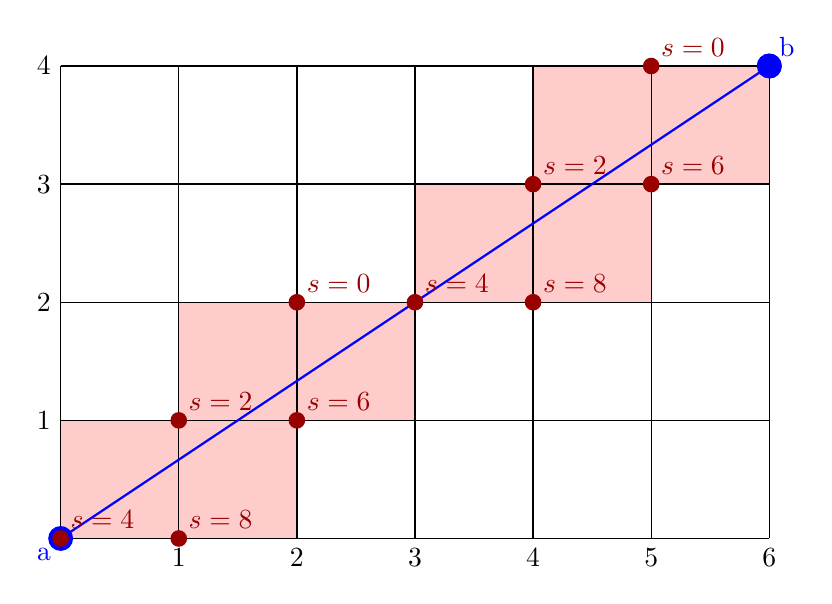
\begin{tikzpicture}[scale=1.5,line width=0.5pt]
    \draw (0,0) grid (6,4);

    \node[below left, blue] at (0,0) {a};
    \node[below] at (1,0) {1};
    \node[below] at (2,0) {2};
    \node[below] at (3,0) {3};
    \node[below] at (4,0) {4};
    \node[below] at (5,0) {5};
    \node[below] at (6,0) {6};

    \node[left] at (0,1) {1};
    \node[left] at (0,2) {2};
    \node[left] at (0,3) {3};
    \node[left] at (0,4) {4};
    \node[above right, blue] at (6,4) {b};
    \fill[blue] (6,4) circle (3pt);

    \filldraw[color=black,fill=red!20] (0,0) rectangle (1,1); 
    \filldraw[color=black,fill=red!20] (1,0) rectangle (2,1);
    \filldraw[color=black,fill=red!20] (1,1) rectangle (2,2);
    \filldraw[color=black,fill=red!20] (2,1) rectangle (3,2);
    \filldraw[color=black,fill=red!20] (3,2) rectangle (4,3); 
    \filldraw[color=black,fill=red!20] (4,2) rectangle (5,3);
    \filldraw[color=black,fill=red!20] (4,3) rectangle (5,4);
    \filldraw[color=black,fill=red!20] (5,3) rectangle (6,4);
    
    \draw[blue, thick] (0,0) -- (6,4);
    \fill[blue] (0,0) circle (3pt);
    \fill[blue] (6,4) circle (3pt);
  
    \node[above right,red!60!black] at (0,0) {$s=4$}; \fill[red!60!black] (0,0) circle (2pt);
    \node[above right,red!60!black] at (1,0) {$s=8$}; \fill[red!60!black] (1,0) circle (2pt);
    \node[above right,red!60!black] at (1,1) {$s=2$}; \fill[red!60!black] (1,1) circle (2pt);
    \node[above right,red!60!black] at (2,1) {$s=6$}; \fill[red!60!black] (2,1) circle (2pt);
    \node[above right,red!60!black] at (2,2) {$s=0$}; \fill[red!60!black] (2,2) circle (2pt);
    \node[above right,red!60!black] at (3,2) {$s=4$}; \fill[red!60!black] (3,2) circle (2pt);
    \node[above right,red!60!black] at (4,2) {$s=8$}; \fill[red!60!black] (4,2) circle (2pt);
    \node[above right,red!60!black] at (4,3) {$s=2$}; \fill[red!60!black] (4,3) circle (2pt);
    \node[above right,red!60!black] at (5,3) {$s=6$}; \fill[red!60!black] (5,3) circle (2pt);
    \node[above right,red!60!black] at (5,4) {$s=0$}; \fill[red!60!black] (5,4) circle (2pt);

  \end{tikzpicture}
  \caption[{\em Line of Sight algorithm}]{Cells checked by the {\em Line of Sight algorithm}, where $\Delta i = 6$ and $\Delta j = 4$} \label{fig:lineofsight}
\end{figure}

\begin{algorithm}
  \SetAlgoLined\DontPrintSemicolon
  \SetKwFunction{los}{LineOfSight}
  \SetKwProg{myDef}{def}{}{}
  \myDef{\los($a$,$b$)}{
    \nl $ i \gets a.x$\;
    \nl $ j \gets a.y$\;
    \nl $ i_{b} \gets b.x$\;
    \nl $ j_{b} \gets b.y$\;
    \nl $ \Delta x \gets i_{b} - i$\;
    \nl $ \Delta y \gets j_{b} - j$\;
    \nl $ s \gets 0$\;
    \nl \While{$i \neq i_{b}$} {
      \nl $s \gets s + \Delta y$\;
      \nl \uIf{$i \geq \Delta i$} {
        \nl \uIf{$cell_{i,j}.isBlocked()$} {
          \nl \KwRet{$false$}\;
        }
        \nl $j \gets j+1$\;
        \nl $s \gets s - 1$\;
      }
      \nl \uIf{$s \neq 0 \land cell_{i,j}.isBlocked()$} {
        \nl \KwRet{$false$}\;
      }
      \nl \uIf{$\Delta j= 0 \land cell_{i,j}.isBlocked() \land cell_{i,j-1}.isBlocked()$} {
        \nl \KwRet{$false$}\;
      }
      \nl $i \gets i + 1$\;
    }
    \nl \KwRet{$true$}\;
  }
  \caption{{\sc LineOfSight}}
\end{algorithm} 

\section{Algorithm Data}
The system uses a {\tt MapInstance} object to encapsulate the concept of a map (with an associated {\em start} and {\em goal} location), the graph that represents that map, and the paths and path statistics calculated for that map by the pathfinding algorithms.\\

\noindent
Each {\tt MapInstance} has an instance variable to store a {\tt Map} object, an instance variable to store the grid-based {\tt Graph} and visibility {\tt Graph} objects that represent that map\footnote{{\tt Map} and {\tt Graph} objects have been introduced in subsections {\bfseries 3.1.1: Maps} and {\bfseries Graphs}}, and a list of {\tt AlgorithmData} objects to store the paths and path statistics for the any pathfinding algorithms that have been run on this map.\\

\noindent
{\tt AlgorithmData} is an abstract class, and there is a concrete class for each pathfinding algorithm that inherits from {\tt AlgorithmData}. It has an {\em enum} type that denotes which pathfinding algorithm the object is holding data for, a public method {\tt go()} which is called to run the pathfinding algorithm, and getter methods which return statistical data about the path found by the pathfinding algorithm. {\tt go()} calculates some of the statistics as follows:

\begin{description}
\item {\bf Path exists}\\ \hfill
whether or not the pathfinding algorithm found a valid path between the {\em start} and {\em goal};
\item {\bf Path length}\\ \hfill
the sum of the Euclidean distances between each pair of consecutive nodes in the path;
\item {\bf Cumulative path angle}\\ \hfill
the sum of the scalar product between each pair of adjacent path segments in the path;
\item {\bf Graph calculation time}\\ \hfill
{\tt System.nanoTime()} is used to calculate the duration between the call to {\tt generateGraph()} and {\tt generateGraph()} returning;
\item {\bf Path calculation time}\\ \hfill
{\tt System.nanoTime()} is used to calculate the duration between the call to {\tt getPath()} and {\tt getPath()} returning;
\item {\bf Number of nodes expanded}\\ \hfill
the number of nodes that were expanded by the pathfinding algorithm.
\end{description}

\begin{figure}
\centering
\begin{tikzpicture} [scale=1.2]
\umlsimpleclass{MapInstance} 
\umlsimpleclass[x=-4,y=-2.5]{Map} 
\umlsimpleclass[x=0,y=-2.5]{Graph}
\umlsimpleclass[x=4,y=-2.5,type=abstract]{AlgorithmData}
\umlsimpleclass[x=-4,y=-5]{Cell} 
\umlsimpleclass[x=0,y=-5]{Node} 
\umlsimpleclass[x=-2,y=-7.5]{Coordinate} 
%\umlclass[x=4,y=-3,type=abstract]{AlgorithmData}{- distance : $double$ \\ - angle : $double$ \\ - path : $List<Coordinate>$ \\ ...}{+ go() : void \\ \# getPath($graph : Graph$) : $Node$ \\ ...} 
\umlHVuniassoc[arg1=1, pos1=0.2, align1=left,arg2=1, pos2=2, align2=right]{MapInstance}{Map}
\umluniassoc[arg1=1, pos1=0.3, align1=right,arg2=2, pos2=1, align2=right]{MapInstance}{Graph}
\umlHVuniassoc[arg1=1, pos1=0.2, align1=right, arg2=7, pos2=2, align2=right]{MapInstance}{AlgorithmData}
\umluniassoc[arg1=1, pos1=0.3, align1=right,arg2=*, pos2=1, align2=right]{Map}{Cell}
\umluniassoc[arg1=1, pos1=0.3, align1=right,arg2=*, pos2=1, align2=right]{Graph}{Node}
%\umluniassoc[mult1=1,pos1=0,mult2=*,pos2=1, angle1=-45, angle2=-135, loopsize=3cm]{Node}{Node}
\umluniassoc[mult1=1,pos1=0.1,mult2=*,pos2=0.9, angle1=45, angle2=-45, loopsize=3cm]{Node}{Node}
\umlVHuniassoc[arg1=1, pos1=0.2, align1=left,arg2=1, pos2=2, align2=right]{Cell}{Coordinate}
\umlVHuniassoc[arg1=1, pos1=0.2, align1=right,arg2=1, pos2=2, align2=left]{Node}{Coordinate}
\end{tikzpicture}
\caption{Composition of {\tt MapInstance}}
\end{figure}

\section{Pathfinding algorithms}
To emphasise the close relationships between the algorithms and to allow for maximum code re-use, the concrete classes that implement the algorithms are arranged in a hierarchy that closely reflects the relationship between the classes, as illustrated in figure 3.5. However, despite {\em Block A*} having a similar basic structure to {\em A*}, a compromise had to be made by having {\em Block A*} inheriting directly from {\em AlgorithmData} as the actual implementation of {\em Block A*} was too different from {\em A*} to allow any meaningful inheritance in the code.\\

\noindent
The inheritance caused by the hierarchy also ensured that any performance differences between algorithms was due to the different nature of each algorithm and not different implementation of similar concepts.\\

\begin{figure}
\centering
\begin{tikzpicture} [scale=1]
\umlemptyclass[type=abstract]{AlgorithmData}
\umlemptyclass[x=-2,y=-3]{Dijkstra}
\umlemptyclass[x=2,y=-3]{BlockAStar}
\umlemptyclass[x=-2,y=-6]{AStar}
\umlemptyclass[x=-2,y=-9]{AStarSmoothed}
\umlemptyclass[x=2,y=-9]{ThetaStar}
\umlemptyclass[x=2,y=-12]{LazyThetaStar}
\umlVHVreal{Dijkstra}{AlgorithmData}
\umlVHVreal{BlockAStar}{AlgorithmData}
\umlVHVinherit{AStar}{Dijkstra}
\umlVHVinherit{AStarSmoothed}{AStar}
\umlVHVinherit{ThetaStar}{AStar}
\umlVHVinherit{LazyThetaStar}{ThetaStar}

\end{tikzpicture}
\caption{Inheritance structure of algorithm implementations}
\end{figure}

\noindent
The remainder of this section will explain the decisions and strategies employed when implementing the pathfinding algorithms.

\subsection{Dijkstra's shortest paths}
The implementation is based on the pseudo-code seen in {\bfseries Algorithm 1} in the {\bfseries Preparation} chapter. By using the {\tt Graph} and {\tt Node} classes introduced in subsections {\bfseries 3.2.1: Graphs}, the translation from pseudo-code to {\em Java} code is transparent. The notable implementation decisions are detailed below:
\begin{description}
  \item {\bf Open Set}\\ \hfill
  the standard {\tt java.util.PriorityQueue} does not automatically re-sort the queue when the priority of an element is changed. Therefore, the algorithm manually {\tt pop()}s, {\tt update()}s and re-{\tt add()}s any node that needed to be updated when already in the {\tt openSet}.
  \item {\bf Closed set}\\ \hfill
  the only two operations on the {\tt closedSet} are adding and checking for membership. Therefore, a {\tt HashSet} is used for its average case O(1) insertion and search speed.
  \item {\bf Extensibility} \\ \hfill
  to allow the clear algorithm hierarchy shown in figure 3.5, {\tt Dijkstra} (i.e. the implementation of {\em Dijkstra}) includes a call to two methods which are required by algorithms that inherit from {\tt Dijkstra}, but are not actually needed by {\tt Dijkstra} itself. The first is {\tt initialise(Node n)} which is called when a node {\tt n} is popped from the {\tt openSet} (which is used by {\em Lazy Theta*}), and the second is a {\tt postProcessing(Node n)} step before the goal node is returned (which is used by {\em A* with post-processing}). In {\tt Dijkstra}  these methods have empty bodies, but some of the algorithms that inherit from {\tt Dijkstra} override these methods.
  \end{description}

\subsection{A*}
{\tt AStar} inherits from {\tt Dijkstra}, and only overrides the {\tt updateCost()} method in accordance with the pseudo-code seen in {\bfseries Algorithm 2} in the {\bfseries Preparation} chapter. 

\subsection{A* with post-smoothing}

{\tt AStarPostSmoothing} inherits from {\tt AStar}, and implements the post-smoothing by only overriding the {\tt postProcessing()}, method which had an empty body in {\tt Dijkstra} and {\tt AStar}. As per the majority of the implementations of {\tt Dijkstra} and {\tt AStar}, the code required for the implementation of {\tt AStarPostSmoothing} is a transparent translation of the pseudo-code presented in {\bfseries Algorithm 3} in the {\bfseries Preparation} chapter.\\

\subsection {Theta* and Lazy Theta*}

The implementations are based on the pseudo-code seen in {\bfseries Algorithm 4} and {\bfseries Algorithm 5} in the {\bfseries Preparation} chapter: 
\begin{description}
\item{\bfseries Theta*}\\ \hfill inherits from {\tt AStar}, and only overrides the {\tt updateCost()} method. {\tt ThetaStar} uses the implementation of the {\em Line of Sight algorithm} introduced in subsection {\bfseries 3.2.4: Line of Sight algorithm}.
\item {\bfseries Lazy Theta*}\\ \hfill inherits from {\tt ThetaStar}, and overrides the {\tt initialiseNode()} and {\tt updateCost()} methods. Note that {\tt LazyThetaStar} is the only class to implement {\tt initialiseNode()}.
\end{description}

\subsection {Block A*}
The implementation of {\em Block A*} is by far the most complex, and hence interesting, of all of the pathfinding algorithms. This is partly because {\em Block A*} is the most intricate of the pathfinding algorithms, and partly because {\em Yap's} paper left large parts of the implementation details unspecified. This provides an opportunity to investigate some different implementation strategies which are described in this section, and compared for efficiency and performance in the {\bfseries Evaluation} chapter.\\

\noindent
{\bfseries LDDB - overview}\\
\noindent
As a reminder for the reader, subsection {\bfseries 2.2.8: Block A*} defines a Local Distance Database $LDDB$ for block size $N^{2}$ as ``$LDDB_{N}$ , a pre-computed database that holds the path length and inflection points of the optimum paths between all pairs of locations $(a,b)$ and $(c,d)$ for all map configurations $M$ of size $N^{2}$, where $a,b,c,d \in \mathbb{Z}$ and $(a,b)$ and $(c,d)$ lie on the boundary of $M$''. {\em Block A*} uses this database of precomputed path lengths to avoid explicitly calculating the paths, and hence the expansion of blocks is faster (since each block expansion requires the knowledge of shortest paths between {\em ingress-egress} pairs of coordinates that lie on the boundary of the block).\\

\noindent
Since there is no publicly available library containing $LDDB$s for {\em Block A*}, the first challenge was to create the $LDDB$s. Although {\em Block A*} only uses a $LDDB$ of a single block size for any one run, multiple $LDDB$s were required for this project so that the performance tradeoffs between $LDDB$s of different block sizes could be investigated. By definition, an $LDDB$ is applicable to any map, so the $LDDB$s only needed to be calculated once for each block size\footnote{As explained later in this section, the three block sizes that are investigated in this project are $2 \times 2$, $3 \times 3$ and $4 \times 4$, so only 3 $LDDB$s were required: $LDDB_{2}$, $LDDB_{3}$ and $LDDB_{4}$.}. Although it is possible to calculate the entries manually for the $LDDB_{2}$, this would certainly not have been feasible for block sizes that were any larger that $2 \times 2$, since for blocks of size {$N \times N$} there will be $2^{N^{2}}$ possible blocks each with $4.N.4.(N-1)$ pairs of $ingress$ and $egress$ coordinates, which gives over 49 thousand optimal path calculations for a block size of $3 \times 3$, and over 12 million optimal path calculations for a block size of $4 \times 4$.\\

\noindent
Therefore, a method was required to create the $LDDB$s automatically. For a given block size $N$, $LDDB_{N}$ contains:\\
(1) \indent for every possible map of size $N^{2}$\\
(2) \indent \indent for every possible $ingress-egress$ coordinate pair\\
(3a) \indent \indent \indent the shortest path between that pair\\
(3b) \indent \indent \indent a list containing every intermediate coordinate on that path.\\

\noindent
The above steps were implemented as follows:
\begin{description}
\item (1) a map of size $N^{2}$ can be represented as a binary integer of $N^{2}$ bits, where each bit represents a cell in the map, and that cell is blocked if the corresponding bit is 0 and is free if the bit is 1. Therefore every possible map of size $N^{2}$ is enumerated by converting each integer from $0$ to $2^{N^{2}}-1$ to the corresponding map representation.\missingfigure{simple figure showing encoding}
\item (2) the possible $ingress$ and $egress$ coordinates are the locations of all nodes that lie on the boundary of a block --- that is to say, all nodes whose coordinates are $(i,j)$, where $[(i=0 \lor i=N) \land (0\leq j \leq N)] \lor [(0\leq i \leq N) \land (j-0 \lor j=N)]$. Therefore, every possible $ingress-egress$ coordinate pair is enumerated by looping over every possible $egress$ coordinate for every possible $ingress$ coordinate.
\item (3) Subsection {\bfseries 2.1.3: The any-angle pathfinding problem} explains that an optimal path in a visibility graph corresponds to the optimal path through the map that the graph represents, and subsection {\bfseries 2.2.4 A*} explains that {\em A*} finds optimal paths through graphs. Therefore, the optimal path through a map between a given $ingress-egress$ coordinate pair is found by converting the map to a visibility graph, and then finding the optimal path through it with {\em A*} (with $ingress = start$ and $egress=goal$. The length required by (3a) is the final value of $n_{goal}.g$, and the list of intermediate coordinates is found by removing the coordinates of $start$ and $goal$ from the list of coordinates in the path returned by {\em A*}.
\end{description}

\noindent
{\bfseries LDDB - uncompressed implementation}\\
\noindent
It is necessary to store the paths and intermediates nodes calculated in steps (3a) and (3b) into a database structure that is compact in memory (so that as much of it as possible can fit into cache) and fast to load and query. Since these constraints are fundamental to the operation of the algorithm, any library or 3\textsuperscript{rd} party database implementation can not be guaranteed to be sufficiently specialised for the task, so a custom database is implemented using arrays and hash tables to ensure optimal performance and minimum space wastage.\\

\noindent
Queries to the database require arguments that describe the configuration of the block (i.e. the configuration of the sub-map that the block represents), and an $ingress-egress$ coordinate pair. Query results are either the length of the shortest path between those nodes, i.e. (3a), or a list of the intermediate coordinates on the shortest path between those the $ingress$ and the $egress$, i.e. (3b).\\

\noindent
Using an actual {\tt Map} object as the query argument to describe the configuration of the block is unnecessarily expensive, as a {\tt Map} object is composed of a square array of {\tt Cell} objects, which are all stored separately on the heap. Therefore, the simple bitwise scheme described in step (2) of {\bfseries LDDB - initial implementation} is used to describe the configuration of a block, and the 32 bits of the {\em Java} {\tt int} primitive is sufficient to encode all possible block configurations of all the block sizes $N$ that are considered in this project: $N=2, 3, 4$\footnote{The reasons for this are explained in the {\bfseries Evaluation} chapter.}. This encoding scheme has dual benefits:
\begin{itemize}
\item the encoded integers are a small (32 bit) value that can be cheaply stored within the {\tt Block} object itself;
\item since these encoded integers form a sequential sequence, they allow the $LDDB_{N}$ to be implemented as an array of size $2^{N^{2}}-1$ which can be indexed by using the encoded integer. This is advantageous as arrays are the most efficient storage format in terms of space and random-access time, which is required by this database.
\end{itemize}

\noindent
Since the $ingress-egress$ coordinate pairs do not fill a sequential space, it would be spatially inefficient to have these coordinate pairs indexing into an array as the array would be very sparse. Therefore, the $ingress-egress$ coordinate pairs index into a hash table, which provides relatively fast random access and space-efficiency for a non-sequential, non-uniform key space.\\

\noindent
Therefore the underlying implementation of the uncompressed implementation database is an array of {\tt  HashMaps} - one {\tt HashMap} per sub-map configuration, with the array indexed by the encoded integer that represents the block. Each {\tt HashMap} maps a key: a {\tt Pair} of $ingress-egress$ {\tt Coordinate}s, to a value: a {\tt Pair} consisting of the length (as a {\tt double}) of the shortest path between the $ingress$ and the $egress$, and an {\tt ArrayList} of the intermediate {\tt Coordinate}s on that path.\\

\begin{figure}
    \centering
    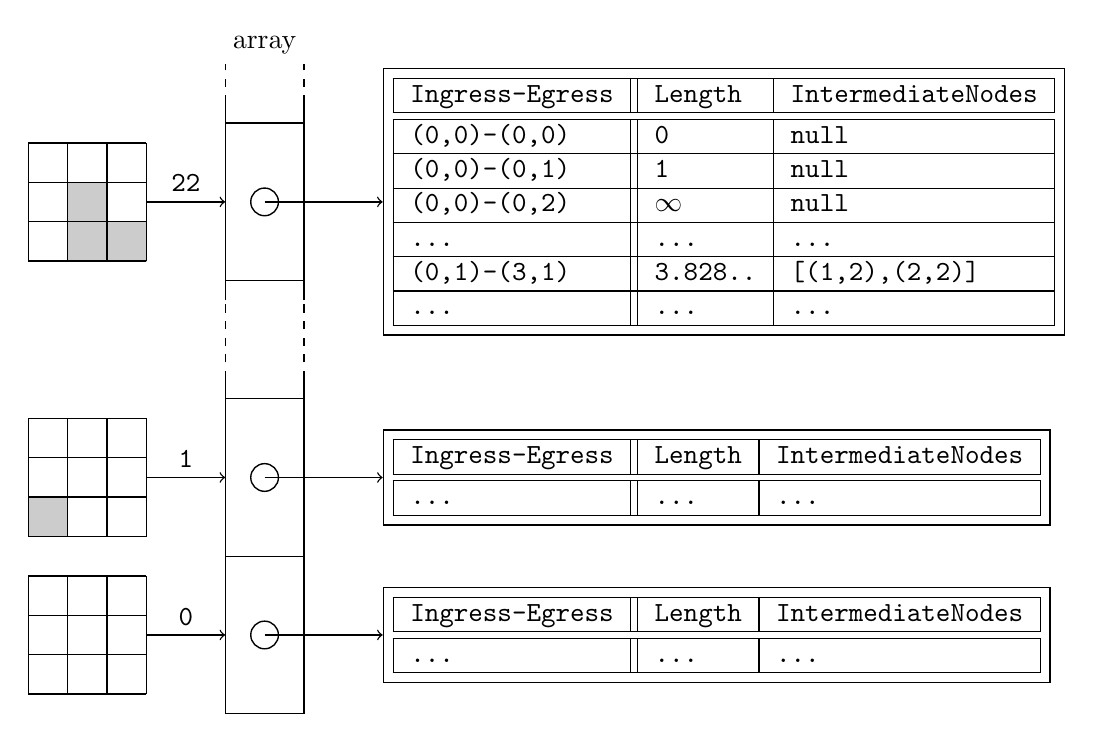
\begin{tikzpicture}[scale=0.5,line width=0.5pt]
    
    \filldraw[black!20] (0,4) rectangle (1,5);
    
    \filldraw[black!20] (1,11) rectangle (2,13);
    \filldraw[black!20] (2,11) rectangle (3,12);
    
      \draw (0,0) grid (3,3);
      \draw (0,4) grid (3,7);
      \draw (0,11) grid (3,14);
      
      \draw (5,-0.5) -- (5,8);
      \draw[dashed] (5,8) -- (5,10);
      \draw(5,10) -- (5,15);
      \draw[dashed] (5,15) -- (5,16);
      \draw (7,-0.5) -- (7,8);
      \draw[dashed] (7,8) -- (7,10);
      \draw(7,10) -- (7,15);
      \draw[dashed] (7,15) -- (7,16);
      
      \draw (5,-0.5) -- (7,-0.5);
      \draw (5,3.5) -- (7,3.5);
      \draw (5,7.5) -- (7,7.5);
      \draw (5,10.5) -- (7,10.5);
      \draw (5,14.5) -- (7,14.5);
      
      \draw[->] (3,1.5) -- (5,1.5);
      \draw[->] (3,5.5) -- (5,5.5);
      \draw[->] (3,12.5) -- (5,12.5);
      
      \node[above] at (4,1.5) {\tt 0};
      \node[above] at (4,5.5) {\tt 1};
      \node[above] at (4,12.5) {\tt 22};
      \node[above] at (6,16) {array};
      
      \draw[->] (6,1.5) -- (9,1.5);   
      \draw (6,1.5) circle (10pt);
      \node[right,draw=black,shape=rectangle] at (9,1.5) (1) {
      \begin{tabular}{| l || l | l |}
    \hline
    {\tt Ingress-Egress} & {\tt Length} & {\tt IntermediateNodes}  \\ \hline \hline
    {\tt ...}  & {\tt ...} & {\tt ...} \\ \hline
    \end{tabular}};
      \draw[->] (6,5.5) -- (9,5.5);
      \draw (6,5.5) circle (10pt);
      \node[right,draw=black,shape=rectangle] at (9,5.5) (1) {
            \begin{tabular}{| l || l | l |}
    \hline
    {\tt Ingress-Egress} & {\tt Length} & {\tt IntermediateNodes}  \\ \hline \hline
    {\tt ...}  & {\tt ...} & {\tt ...} \\ \hline
    \end{tabular}};
      \draw[->] (6,12.5) -- (9,12.5);
      \draw (6,12.5) circle (10pt);
      \node[right,draw=black,shape=rectangle] at (9,12.5) (1) {
    \begin{tabular}{| l || l | l |}
    \hline
    {\tt Ingress-Egress} & {\tt Length} & {\tt IntermediateNodes}  \\ \hline \hline
    {\tt (0,0)-(0,0)}  & {\tt 0} & {\tt null} \\ \hline
    {\tt (0,0)-(0,1)}  & {\tt 1} & {\tt null} \\ \hline
    {\tt (0,0)-(0,2)}  & {\tt $\infty$} & {\tt null} \\ \hline
    {\tt ...}  & {\tt ...} & {\tt ...} \\ \hline
    {\tt (0,1)-(3,1)}  & {\tt 3.828..} & {\tt [(1,2),(2,2)]} \\ \hline
    {\tt ...}  & {\tt ...} & {\tt ...} \\ \hline
\end{tabular}};
      

    \end{tikzpicture}
  \caption[Extract of the uncompressed implementation of $LDDB_{3}$]{Extract of the uncompressed implementation of $LDDB_{3}$, detailing part of the {\tt HashTable} for the block configuration with an encoded integer representation of 22.}
  %\label{fig:fig}
\end{figure}

\noindent
{\bfseries LDDB --- compressed implementation}\\
\noindent
The uncompressed implementation of the database has the advantage that the query arguments and result values are in the same data format that is used by the algorithm, and hence there is a no overhead in converting the data to/from a different format. However due to the fact that the size of a database $LDDB_{N}$ increases exponentially as block size $N$ increases, the uncompressed implementation of $LDDB_{4}$ is large, which causes slow loading to memory, less of the $LDDB$ stored in cache and a higher likelihood of thrashing during execution. Therefore, an implementation was devised that makes use of two further bitwise encoding schemes:
\begin{enumerate}
\item each {\tt Pair} of ingress-egress {\tt Coordinate}s can be represented with a unique integer representable in a {\tt byte}'s worth of space. An efficient hash function was devised to convert from a {\tt PairOfCoordinate} object to this encoded byte representation. The encoding scheme is given in Figure 3.7;
\item the {\tt List} of intermediate {\tt Coordinate}s can be represented by a unique code that fits into the 32 bits of an integer, since: the maximum number of intermediate nodes on a shortest path in a sub-map of size up to {$N=4$} is 4\footnote{Obtained by experimental results.}, and the range of $x$ and $y$ in each {\tt Coordinate} in a sub-map of size up to {$N=4$} is 0-4, therefore 6 bits can be used for each {\tt Coordinate}: 3 for $x$ (as 3 bits has sufficient capacity to represent the range 0-4), 3 for $y$, which is a maximum total of 4*6 = 24 bits. The encoding scheme is given in Figure 3.8.
\end{enumerate}

\noindent 
Therefore, if {\em Block A*} uses a compressed $LDDB$, each query requires encoding the block configuration (as described in the uncompressed implementation) and the $ingress-egress$ coordinate pair (which is the first of the two bitwise encoding schemes introduced above). If the query result is the length of a shortest path then no decoding is required, but if the result is the intermediate nodes on shortest path then this result must be decoded from the scheme described in the second of the two bitwise encoding schemes introduced above. Therefore in comparison to the uncompressed implementation, the compressed implementation has the advantage of smaller space requirements, but it has the disadvantage that each query requires encoding and some results require decoding.

\begin{figure}
\begin{lstlisting}
PairOfCoords(Coordinate c1, Coordinate c2, int blockSize) {
		this.blockSize = blockSize;
		this.coordCode = (byte) 
			(c1.getX() + 
			c1.getY() * (blockSize+1) + 
			c2.getX() * (blockSize+1)*(blockSize+1) + 
			c2.getY() * (blockSize+1)*(blockSize+1)*(blockSize+1));
	}
\end{lstlisting}
\caption{Encoding scheme for {\tt PairOfCoords} in the compressed LDDB}
\end{figure}

\begin{figure}
\begin{lstlisting}
int getListCode(List<Coordinate> intermediateNodes) {
		int listCode = 0;
		for(Coordinate c : intermediateNodes) {
			listCode = listCode | c.getX();
			listCode = listCode << 3;
			listCode = listCode | c.getY();
			listCode = listCode << 3;
		}
		listCode = listCode >>> 3;	//undoes line 7 on final loop
		return listCode;
	}
\end{lstlisting}
\caption{Encoding scheme for {\tt List<Coordinate>} in the compressed LDDB}
\end{figure}

\noindent
{\bfseries LDDB --- super-compressed implementation}\\
\noindent
The compressed implementation of the database uses bitwise encoding schemes to compress the database. Further compressions are possible by taking advantage of the fact that:
\begin{enumerate}
\item the shortest path between an $ingress-egress$ pair $a$ and $b$ is the reverse of the shortest path between an $ingress-egress$ pair $b$ and $a$. 
\item some block configurations are 90$^{\circ}$,  180$^{\circ}$ or 270$^{\circ}$ rotations of other block configurations.
\end{enumerate}

These two properties leverage the redundancy in the compressed database as described below:
\begin{enumerate}
\item The data for only one of the two `reflection' pairs of $ingress-egress$ coordinates $a,b$ and $b,a$ needs to be stored in the database, using a simple policy to determine which one of these two pairs is stored. This same policy can be used to determine whether the $ingress-egress$ pair needs to be reversed in a query to the $LDDB$ --- if the $ingress-egress$ pair does need to be reversed in the query, then the intermediate nodes in the query result will also need to be reversed. The policy is that if $a.y < b.y$ or $(a.y = b.y) \land (a.x \leq b.y)$ then the pair will be found as $a,b$ in the database, otherwise they are found as $b,a$.
\item The data for only one of the four rotations of block configuration needs to be stored in the database, using a simple policy  to determine which of the rotations is stored. This same policy can be used to determine whether block configuration needs to be rotated in a query to the $LDDB$ --- if the block configuration does need to be rotated in the query, then the intermediate nodes in the query result will need to be rotated by the same amount in the opposite direction. The policy is that the rotation with the smallest encoded integer representation (as introduced for the uncompressed implementation of the $LDDB$) is the one that is stored. 
\end{enumerate}

\noindent
{\bf Special case blocks}\\

\noindent
As explained in the {\bfseries Blocks} paragraph of {\bfseries 2.2.8: Block A*}, the edge weights for $block_{start}$ and $block_{goal}$ may not be present in the $LDDB$. The $LDDB$ only contains data for paths between $ingress-egress$ pairs of coordinates (where $ingress$ and $egress$ coordinates lie on the boundaries of blocks), yet $start$ and $goal$ are not guaranteed to lie on the boundary of a block. Therefore, alternative methods must be used to obtain the edge weights for $block_{start}$ and $block_{goal}$. Two methods were identified:
\begin{enumerate}
\item {\bfseries compute the edge weights at runtime}, by using a similar method to that which was used to compute the shortest paths contained in the $LDDB$ --- i.e. but generating a visibility graph to represent the sub-map that $block_{start}$, and using {\em A*} to find the shortest path between $n_{start}$ and all boundary nodes of $block_{start}$, and then similarly for $block_{start}$. In the exceptional case that $block_{start} = block_{goal}$, this method can be slightly modified to return the shortest path directly. 
\item{\bfseries extend the LDDB} so that it also includes data for all possible edges in $block_{start}$ and $block_{goal}$. The original, unextended $LDDB$ (regardless of whether it is uncompressed, compressed or super-compressed) contains details of shortest paths from {\em any boundary} node to {\em any boundary} node in a block, so there are two possibilities for extension:
  \begin{enumerate}
  \item{\bf semi-extended $LDDB$} contains details of shortest paths from {\em any} node to {\em any boundary} node in a block. This $LDDB$ will have all data required by {\em Block A*} for all blocks, except for in the exceptional case that $block_{start} = block_{goal}$, in which case a visibility graph of the block must be calculated and solved with {\em A*} as in option (1).
  \item{\bf fully-extended $LDDB$} contains details of shortest paths from {\em any} node to {\em any} node in a block. This $LDDB$ will have all data required by {\em Block A*} for all blocks.
  \end{enumerate} 
\end{enumerate}

\noindent
These three methods (1, 2a and 2b), as well as the different compression implementations all involve tradeoffs between space and time. The performance of {\em Block A*} using these different forms of $LDDB$ will be analysed in the {\bfseries Evaluation} chapter.\\

\noindent
{\bf Algorithm} \\
\noindent
Having carefully set up the problem in the {\bfseries Preparation} chapter, the majority of the implementation of the main part of the algorithm was a transparent translation of the pseudo-code in {\bfseries Algorithm 6} using similar design choices to the other pathfinding algorithms.\\

\noindent
{\bf Traceback} \\
\noindent
The traceback stage, which is unspecified in Yap's paper and the {\bfseries Preparation} chapter, requires explanation. The path $P_{G_{M}}$ is produced by:
\begin{itemize}
\item adding all nodes obtained by recursively following the $parent$ pointers from $n_{goal}$ to $n_{start}$;
\item removing all but one of any set of collocation nodes this occurs when the path crosses block boundaries;
\item adding any intermediate nodes where the path traverses a block --- these are obtained by querying the $LDDB$.
\end{itemize}
 
\section{Visualizer}

The maps and paths are displayed by implementing the {\tt paintComponent()} method of the visualizer panel. The UI also allows the user to display or hide different combinations of paths and which nodes were expanded in the calculation of those paths for all of the different pathfinding algorithms.

\begin{figure}
\centering
\shadowpicture{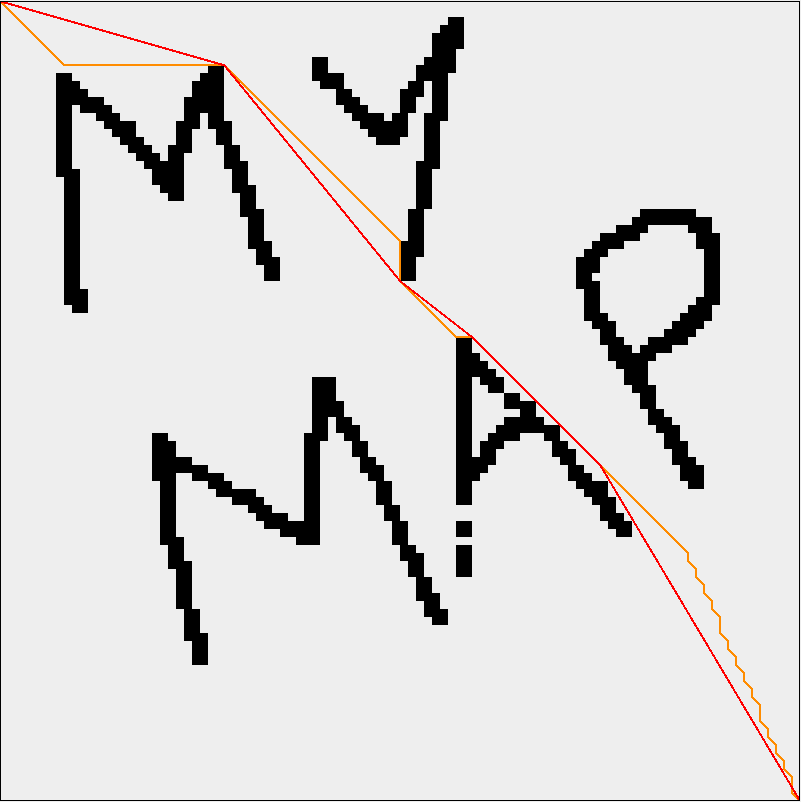
\includegraphics[width=0.8\textwidth]{creationmode.png}}
\caption{User interface in map creation mode}
\end{figure}

\begin{figure}
\centering
\shadowpicture{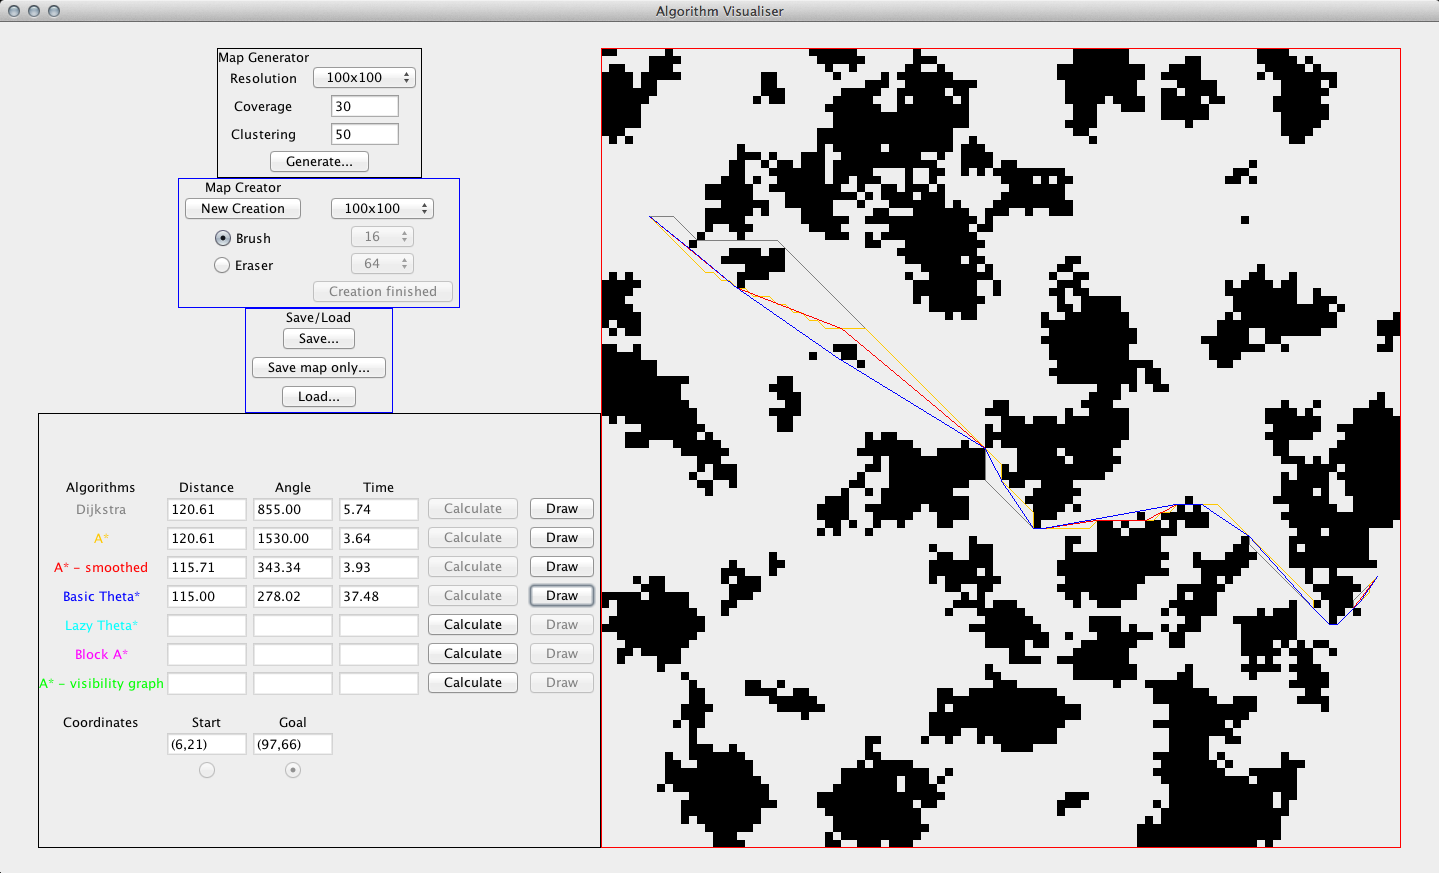
\includegraphics[width=0.8\textwidth]{paths.png}}
\caption{User interface displaying paths for a generated map}
\end{figure}

\section{Testing}

\todo{Implementation: testing \ldots}

\section{Data extraction}

The engine is designed to have a simple API that allows both a UI to be bolted on and scripts that can bypass the UI altogether. The open source package {\tt CSVWriter} is used to write the pathfinding data obtained from the API to CSV files. This data is then processed by $R$ scripts, which parse the imported CSVs into $dataframes$ and apply various statistical analyses to produce the data summarised in the {\bf Evaluation} chapter.

\begin{figure}
\centering
    \begin{tabular}{| l | l | l | l | l |}
    \hline
    Map & Algorithm & PathTime & TotalLength & TotalAngle\\ \hline % & NodesExp\\ \hline
     Map 1 & Dijkstra & 852.926976 & 160.752308679 & 495.0000736525\\ \hline % & 8203\\ \hline
     Map 1 & AStar & 169.831936 & 160.752308679 & 855.0000688228\\ \hline %  & 2999\\ \hline
     Map 1 & AStarVisibility & 5.334016 & 151.6768359881 & 102.262577962\\ \hline %  & 289\\ \hline
Map 1 & AStarSmoothed & 85.908992 & 154.9127142045 & 165.3889464848\\ \hline %  & 2999\\ \hline
Map 1 & ThetaStar & 30.230016 & 151.7637935619 & 122.1222152092\\ \hline %  & 1682\\ \hline
Map 1 & LazyThetaStar & 32.45824 & 151.7637935619 & 122.1222152092\\ \hline %  & 1692\\ \hline
Map 1 & BlockAStar & 10.85792 & 152.8713149055 & 566.7296353554\\ \hline %  & 3278\\ \hline
Map 2 & Dijkstra & 615.220992 & 161.3380951166 & 810.0000676154\\ \hline %  & 8146\\ \hline
 \end{tabular}
\caption{Extract from a CSV file exported by {\tt DataExtract}}
\end{figure}

\begin{figure}
\begin{lstlisting}
void generateMaps 
	(int size, int coverage, int clustering, int numberOfMaps) {
	
	for(int i=0;i<numberOfMaps;i++) {
		saveMapOnly(size+"/"+coverage+"/"+clustering+"/"+i+".ser",
			new MapInstance(
				MapGenerator.generateMap(size,size,coverage,clustering)));
	}
}
\end{lstlisting}
\caption{Code snippet from {\tt DataExtraction} showing automation of {\tt Graph} creation}
\end{figure}

\begin{figure}
    \centering
    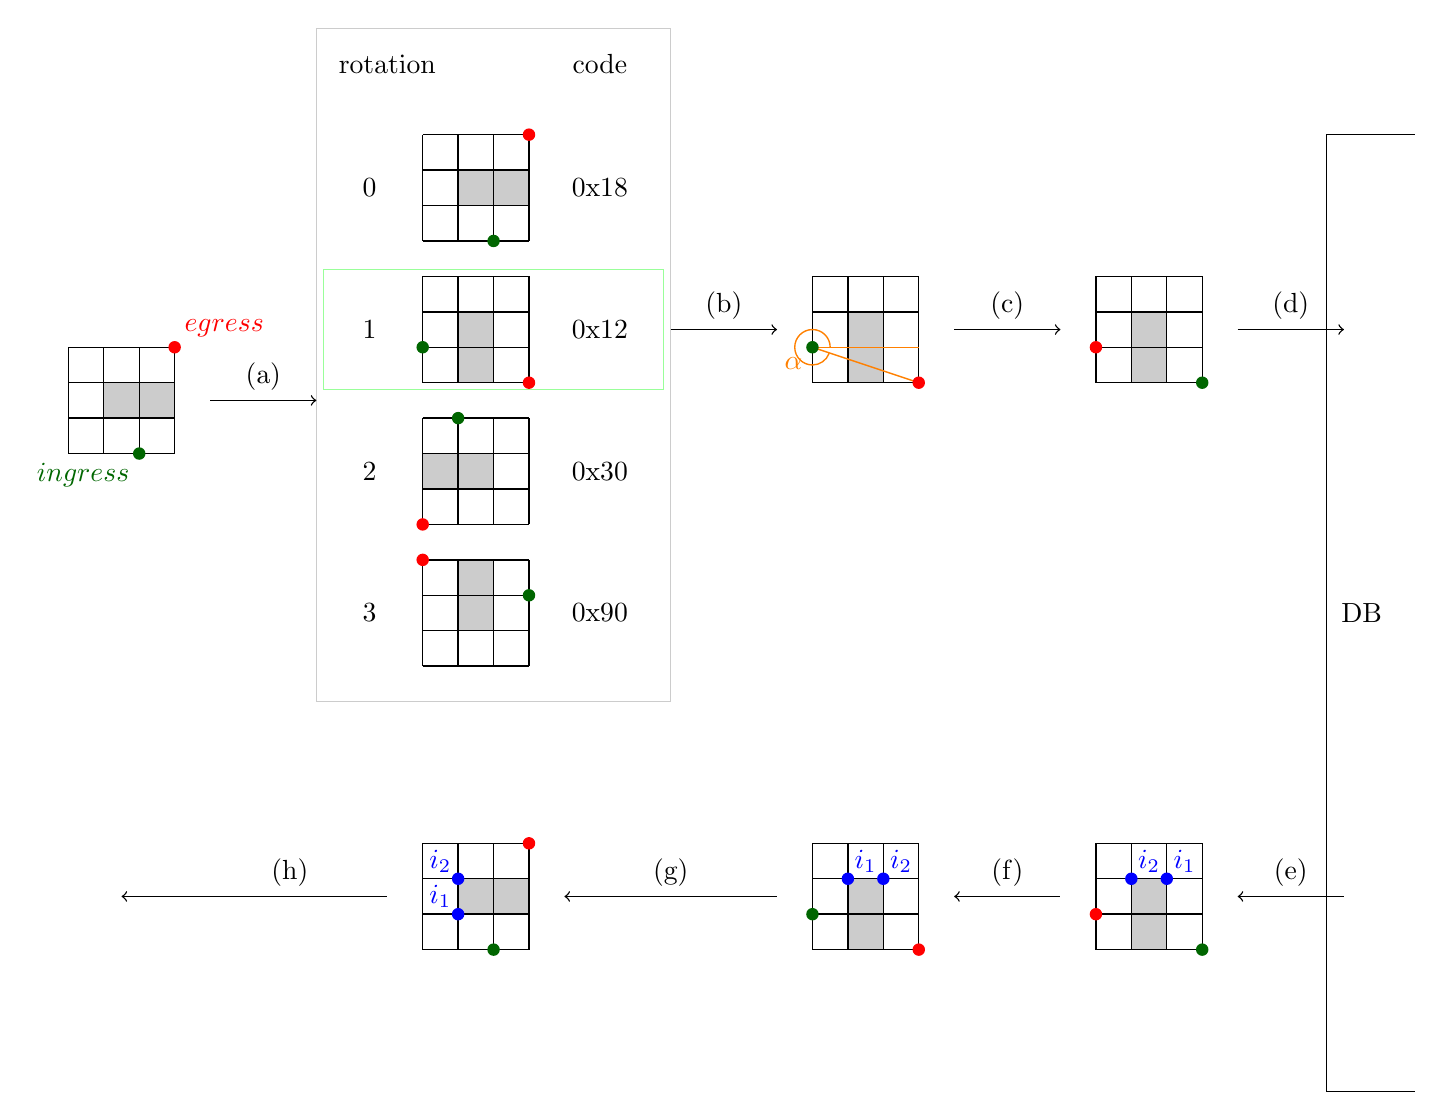
\begin{tikzpicture}[scale=0.45,line width=0.5pt]
    
    %input
    \filldraw[black!20] (-9,7) rectangle (-7,8);
    \draw (-10,6) grid (-7,9);
    \fill[black!60!green] (-8,6) circle (5pt);
    \node[below left, black!60!green] at (-8,6) {$ingress$};
    \fill[red] (-7,9) circle (5pt);
    \node[above right, red] at (-7,9) {$egress$};
    
    %rotations
    \draw[black!20] (-3,-1) rectangle (7,18);
    \draw[green!40] (-2.8,7.8) rectangle (6.8,11.2);
    
    \filldraw[black!20] (1,13) rectangle (3,14);
    \draw (0,12) grid (3,15);
    \fill[black!60!green] (2,12) circle (5pt);
    \fill[red] (3,15) circle (5pt);
        
    \filldraw[black!20] (1,8) rectangle (2,10);
    \draw (0,8) grid (3,11);
    \fill[black!60!green] (0,9) circle (5pt);
    \fill[red] (3,8) circle (5pt);
        
    \filldraw[black!20] (0,5) rectangle (2,6);
    \draw (0,4) grid (3,7);
    \fill[black!60!green] (1,7) circle (5pt);
    \fill[red] (0,4) circle (5pt);
    
    \filldraw[black!20] (1,1) rectangle (2,3);
    \draw (0,0) grid (3,3);
    \fill[black!60!green] (3,2) circle (5pt);
    \fill[red] (0,3) circle (5pt);
    
    \draw[->] (-6,7.5) -- (-3,7.5);
    \node[above] at (-4.5,7.5) {(a)};
    
    \node at (-1,17) {rotation};	\node at (5,17) {code};
    \node at (-1.5,13.5) {0};		\node at (5,13.5) {0x18};
    \node at (-1.5,9.5) {1};		\node at (5,9.5) {0x12};
    \node at (-1.5,5.5) {2};		\node at (5,5.5) {0x30};
    \node at (-1.5,1.5) {3};		\node at (5,1.5) {0x90};
    
    \draw[->] (7,9.5) -- (10,9.5);
    \node[above] at (8.5,9.5) {(b)};
   
   %angle check
    \filldraw[black!20] (12,8) rectangle (13,10);
    \draw (11,8) grid (14,11);
    \draw[orange] (11,9) -- (14,9);
    \draw[orange] (11,9) -- (14,8);
    \draw[orange] (11.5,9) arc (0:340:0.5);
    \node[below left, orange] at (11,9) {$\alpha$};
    \fill[black!60!green] (11,9) circle (5pt);
    \fill[red] (14,8) circle (5pt);
    
    \draw[->] (15,9.5) -- (18,9.5);
    \node[above] at (16.5,9.5) {(c)};
    
    %DB input
    \filldraw[black!20] (20,8) rectangle (21,10);
    \draw (19,8) grid (22,11);
    \fill[red] (19,9) circle (5pt);
    \fill[black!60!green] (22,8) circle (5pt);
    
    \draw[->] (23,9.5) -- (26,9.5);
    \node[above] at (24.5,9.5) {(d)};
    \draw (25.5,15) -- (28,15);
    \draw (25.5,-12) -- (28,-12);
    \draw (25.5,-12) -- (25.5,15);
    \node at (26.5,1.5) {DB};
        
    \draw[<-] (23,-6.5) -- (26,-6.5);
    \node[above] at (24.5,-6.5) {(e)};
    
    %DB output
    \filldraw[black!20] (20,-8) rectangle (21,-6);
    \draw (19,-8) grid (22,-5);
    \fill[red] (19,-7) circle (5pt);
    \fill[black!60!green] (22,-8) circle (5pt);
    \fill[blue] (21,-6) circle (5pt);
    \node[blue] at (21.5,-5.5) {$i_{1}$};
    \fill[blue] (20,-6) circle (5pt);
    \node[blue] at (20.5,-5.5) {$i_{2}$};
    
    \draw[<-] (15,-6.5) -- (18,-6.5);
    \node[above] at (16.5,-6.5) {(f)};
    
    %flipped
    \filldraw[black!20] (12,-8) rectangle (13,-6);
    \draw (11,-8) grid (14,-5);
    \fill[black!60!green] (11,-7) circle (5pt);
    \fill[red] (14,-8) circle (5pt);
    \fill[blue] (12,-6) circle (5pt);
    \node[blue] at (12.5,-5.5) {$i_{1}$};
    \fill[blue] (13,-6) circle (5pt);
    \node[blue] at (13.5,-5.5) {$i_{2}$};
    
    \draw[<-] (4,-6.5) -- (10,-6.5);
    \node[above] at (7,-6.5) {(g)};
    
    %rotated
    \filldraw[black!20] (1,-7) rectangle (3,-6);
    \draw (0,-8) grid (3,-5);
    \fill[black!60!green] (2,-8) circle (5pt);
    \fill[red] (3,-5) circle (5pt);
    \fill[blue] (1,-7) circle (5pt);
    \node[blue] at (0.5,-6.5) {$i_{1}$};
    \fill[blue] (1,-6) circle (5pt);
    \node[blue] at (0.5,-5.5) {$i_{2}$};
    
    \draw[<-] (-8.5,-6.5) -- (-1,-6.5);
    \node[above] at (-3.75,-6.5) {(h)};


    \end{tikzpicture}
  \caption{my caption}
  %\label{fig:fig}
\end{figure}


\chapter{Evaluation}

\begin{center}
    \begin{tabular}{| l | l | l |}
    \hline
    Submap size & Size of uncompressed LDDB & Size of compressed LDDB\footnotemark[3]$^{,}$\footnotemark[4]  \\ \hline
    {$2 \times 2$}  & 33KB  & 17KB \\ \hline
    {$3 \times 3$}  & 2.2MB & 1.1MB \\ \hline
    {$4 \times 4$}  & 485MB & 192MB \\ \hline
  \end{tabular}
\end{center}
\footnotetext[3]{These savings could be improved further for sub maps of size {$2 \times 2$} and {$3 \times 3$} by using specific data-types depending on the submap size, but this was unnecessary, as the LDDB size was very small compared to the total available memory for sub maps of size{$2 \times 2$} and {$3 \times 3$}, and the LDDB only needs to be loaded into memory once per run of the program.}
\footnotetext[4]{These sizes were significantly larger than those found in Yap's paper, but his agents were only allowed to travel horizontally and vertically, so only 4 bits were needed to store the path length value.}

\noindent
The increase in the size of the LDDB in comparison to the original is:
\begin{center}
    \begin{tabular}{| l | l | l |}
    \hline
    Submap size & Semi-extended & Fully-extended  \\ \hline
    {$2 \times 2$}  & 12.5\% & 26.5\% \\ \hline
    {$3 \times 3$}  & 33.3\% & 77.8\%\\ \hline
    {$4 \times 4$}  & 56.3\% & 144.1\% \\ \hline
  \end{tabular}
\end{center}

Text\footnote{Note that when using the semi-extended $LDDB$, $block_{goal}$ needs to reverse the $ingress-egress$ coordinates before querying the LDDB.}.


\chapter{Conclusion}

\bibliography{refs}{}
\bibliographystyle{unsrt}

\appendix




\cleardoublepage

\end{document}